% Settings for the default beamer theme
\documentclass[english, aspectratio=169]{beamer}
\usepackage[T1]{fontenc}
\usepackage[utf8]{inputenc}
\usepackage{tabularx}
\usepackage{babel}
\usepackage[ruled,vlined]{algorithm2e}
\SetAlgorithmName{Algoritmus}{algoritmus}{List of Algorithms}
\setcounter{secnumdepth}{3}
\setcounter{tocdepth}{3}
\definecolor{lightgray}{gray}{0.9}

\makeatletter

\newcommand\makebeamertitle{\frame{\maketitle}}

% (ERT) argument for the TOC
\AtBeginDocument{%
  \let\origtableofcontents=\tableofcontents
  \def\tableofcontents{\@ifnextchar[{\origtableofcontents}{\gobbletableofcontents}}
  \def\gobbletableofcontents#1{\origtableofcontents}
}

% Theme settings
\usetheme{Frankfurt}
\usecolortheme{default}
\usefonttheme[onlymath]{serif}

% Template settings
\setbeamertemplate{navigation symbols}{}
\setbeamertemplate{blocks}[rounded][shadow=false]
\setbeamertemplate{title page}[default][colsep=-4bp, rounded=true, shadow=false]
\makeatother

% Define a custom darker red color
\definecolor{DarkerRed}{RGB}{139,0,0} % Adjust the RGB values as needed

% Use the newly defined color in Beamer theme elements
\setbeamercolor{structure}{fg=DarkerRed} % Changes basic structural elements to Darker Red
\setbeamercolor{title in head/foot}{bg=DarkerRed} % Changes the title in header/footer to Darker Red


\begin{document}

% Title page
\section{Bevezetés}
\title[]{Üzleti Elemzések Módszertana}
\subtitle{2. Előadás: Osztályozás}
\author[Kuknyó Dániel]{Kuknyó Dániel\\Budapesti Gazdasági Egyetem}
\date{2023/24\\2.félév}
\makebeamertitle

% Table of contents slide
\begin{frame}
\tableofcontents{}
\end{frame}

% Table of contents of the current section
\begin{frame}
\tableofcontents[currentsection]
\end{frame}

\begin{frame}{A determinisztikus szemléletmód}
\begin{columns}
\begin{column}{.5\textwidth}
A hagyományos szoftverfejlesztési folyamatmodell eljárása:
\begin{enumerate}
	\item Az adott jelenség megfigyelése és adatok rögzítése
	\item A megfigyelésekre olyan szabályok kidolgozása, amelyek jól leírják azt
	\item A létrejött szabályrendszer kiértékelése
	\item Rendszer fejlesztése a hibák alapján
	\item Iteráció
\end{enumerate}
\end{column}
\begin{column}{.5\textwidth}
\begin{center}
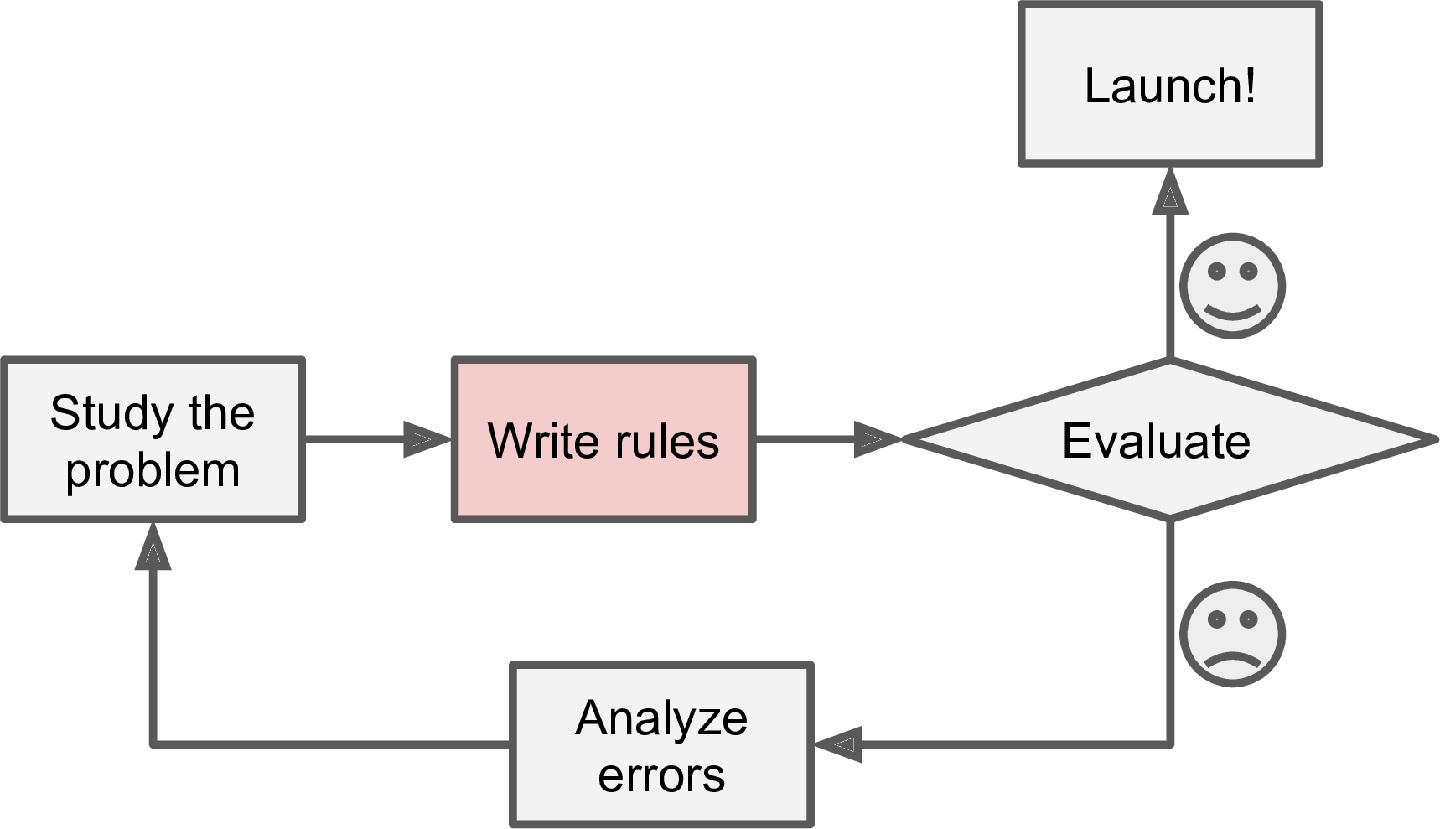
\includegraphics[width=7cm, height=7cm, keepaspectratio]{images/osztalyozas_1.png}
\end{center}
\end{column}
\end{columns}
\end{frame}

\begin{frame}{A gépi tanulás szemléletmód}
\begin{columns}
\begin{column}{.5\textwidth}
A gépi tanulás szemléletének folyamatmodellje:
\begin{enumerate}
	\item Adott jelenség megfigyelése és adatok rögzítése
	\item Gépi tanulási modell tanítása az adatokon a szakterületi tudás segítségével
	\item Modell kiértékelése
	\item Hibák elemzése és kiértékelése
	\item Iteráció
\end{enumerate}
\end{column}
\begin{column}{.5\textwidth}
\begin{center}
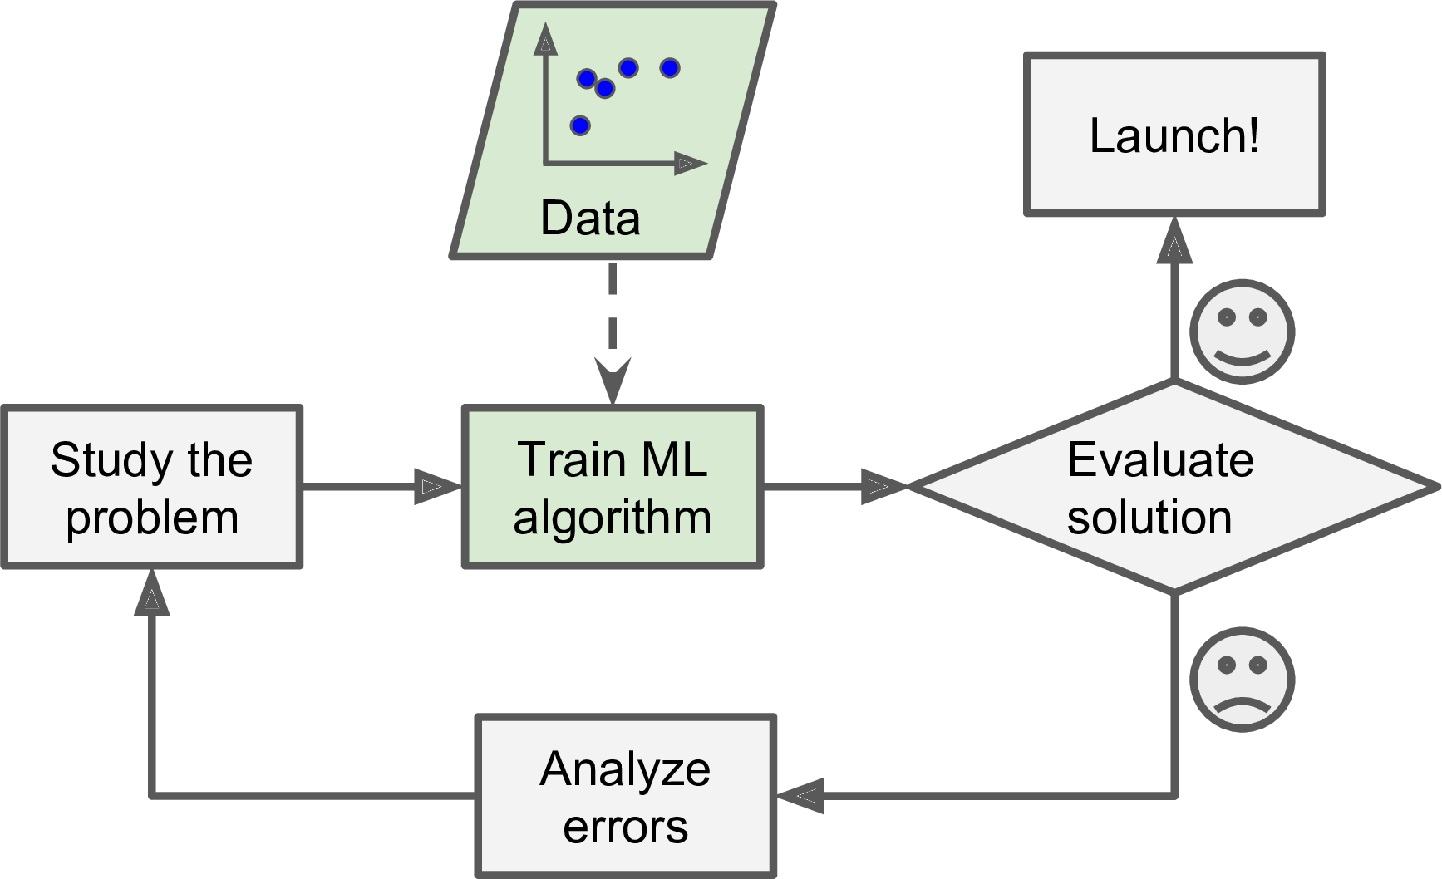
\includegraphics[width=7cm, height=7cm, keepaspectratio]{images/osztalyozas_2.png}
\end{center}
\end{column}
\end{columns}
\end{frame}

\begin{frame}{Tanítás automatizálása adatalapúan}
\begin{columns}
\begin{column}{.5\textwidth}
Az gépi tanuló modellek tanítása és kiértékelése hosszú távon egy iteratív folyamat már létező keretrendszerekkel, mint az MLOps. Ennek számos területen vannak előnyei:
\begin{itemize}
	\item Adaptáció az új adatokhoz
	\item Javuló modell teljesítmény
	\item Hibák és problémák azonosítása
	\item Új technológiai fejlődés integrálása
	\item Skálázhatóság és rugalmasság
	\item Szakterületi következtetések az elemzések által
\end{itemize}
\end{column}
\begin{column}{.5\textwidth}
\begin{center}
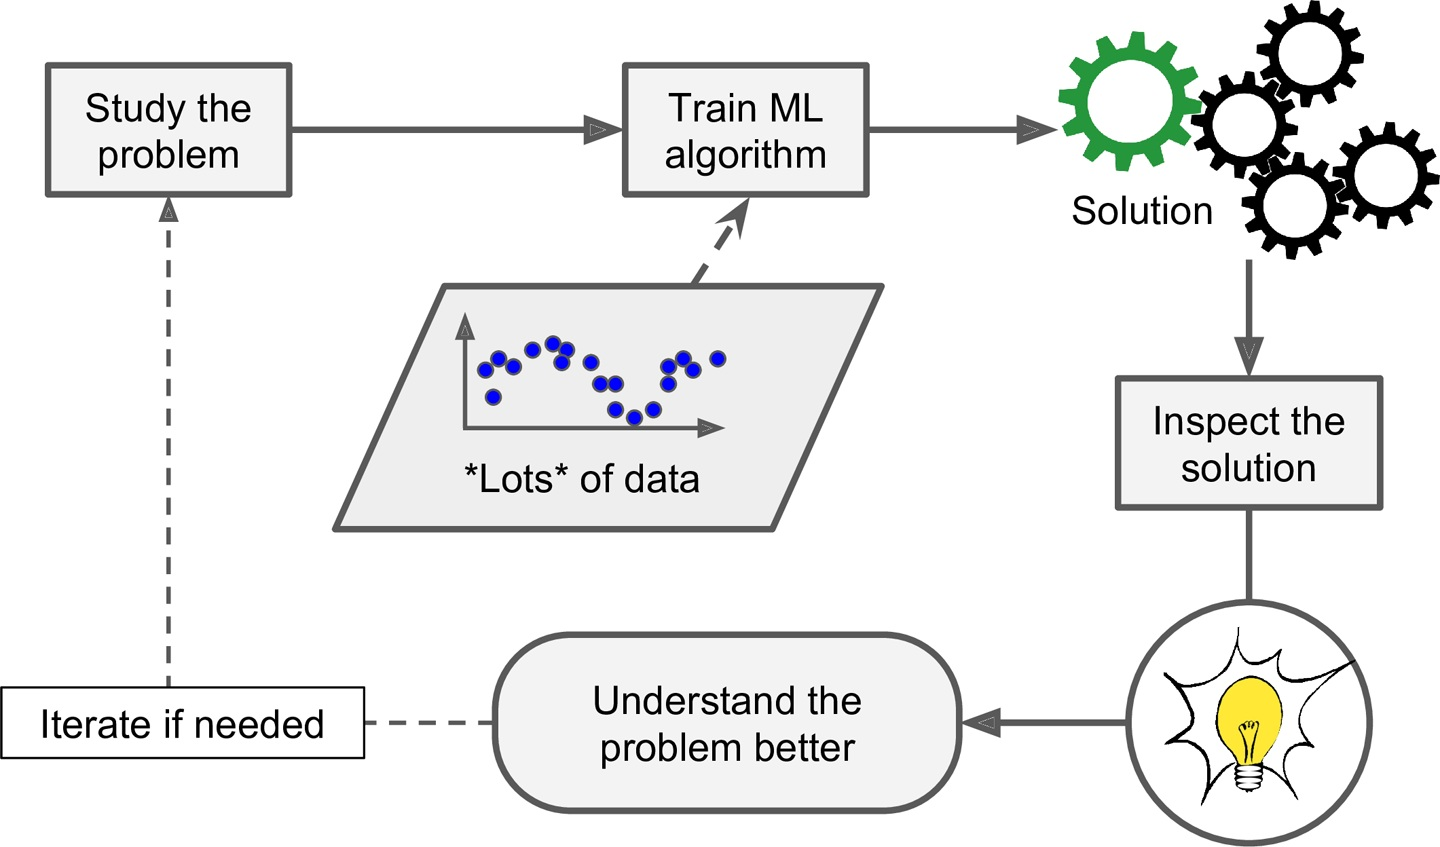
\includegraphics[width=7cm, height=7cm, keepaspectratio]{images/osztalyozas_3.png}
\end{center}
\end{column}
\end{columns}
\end{frame}

\begin{frame}{Az adatok észszerűtlen hatékonysága}
\begin{columns}
\begin{column}{.5\textwidth}
2001-es kutatásukban Michele Blanko és Eric Brill kimutatták, hogy a különböző ML algoritmusok \textbf{hasonlóan jól teljesítenek a természetes nyelvfelismerés területén mint a hagyományos algoritmusok}, ha elég sok adaton tanítják a modelleket. Ahogy ők fogalmaztak:\par\medskip
\emph{„Az eredmények azt mutatják, hogy újra kell gondolnunk, mire fordítjuk a pénzünket és erőforrásainkat: algoritmusok fejlesztésére, vagy adatgyűjtésre.”}
\end{column}
\begin{column}{.5\textwidth}
\begin{center}
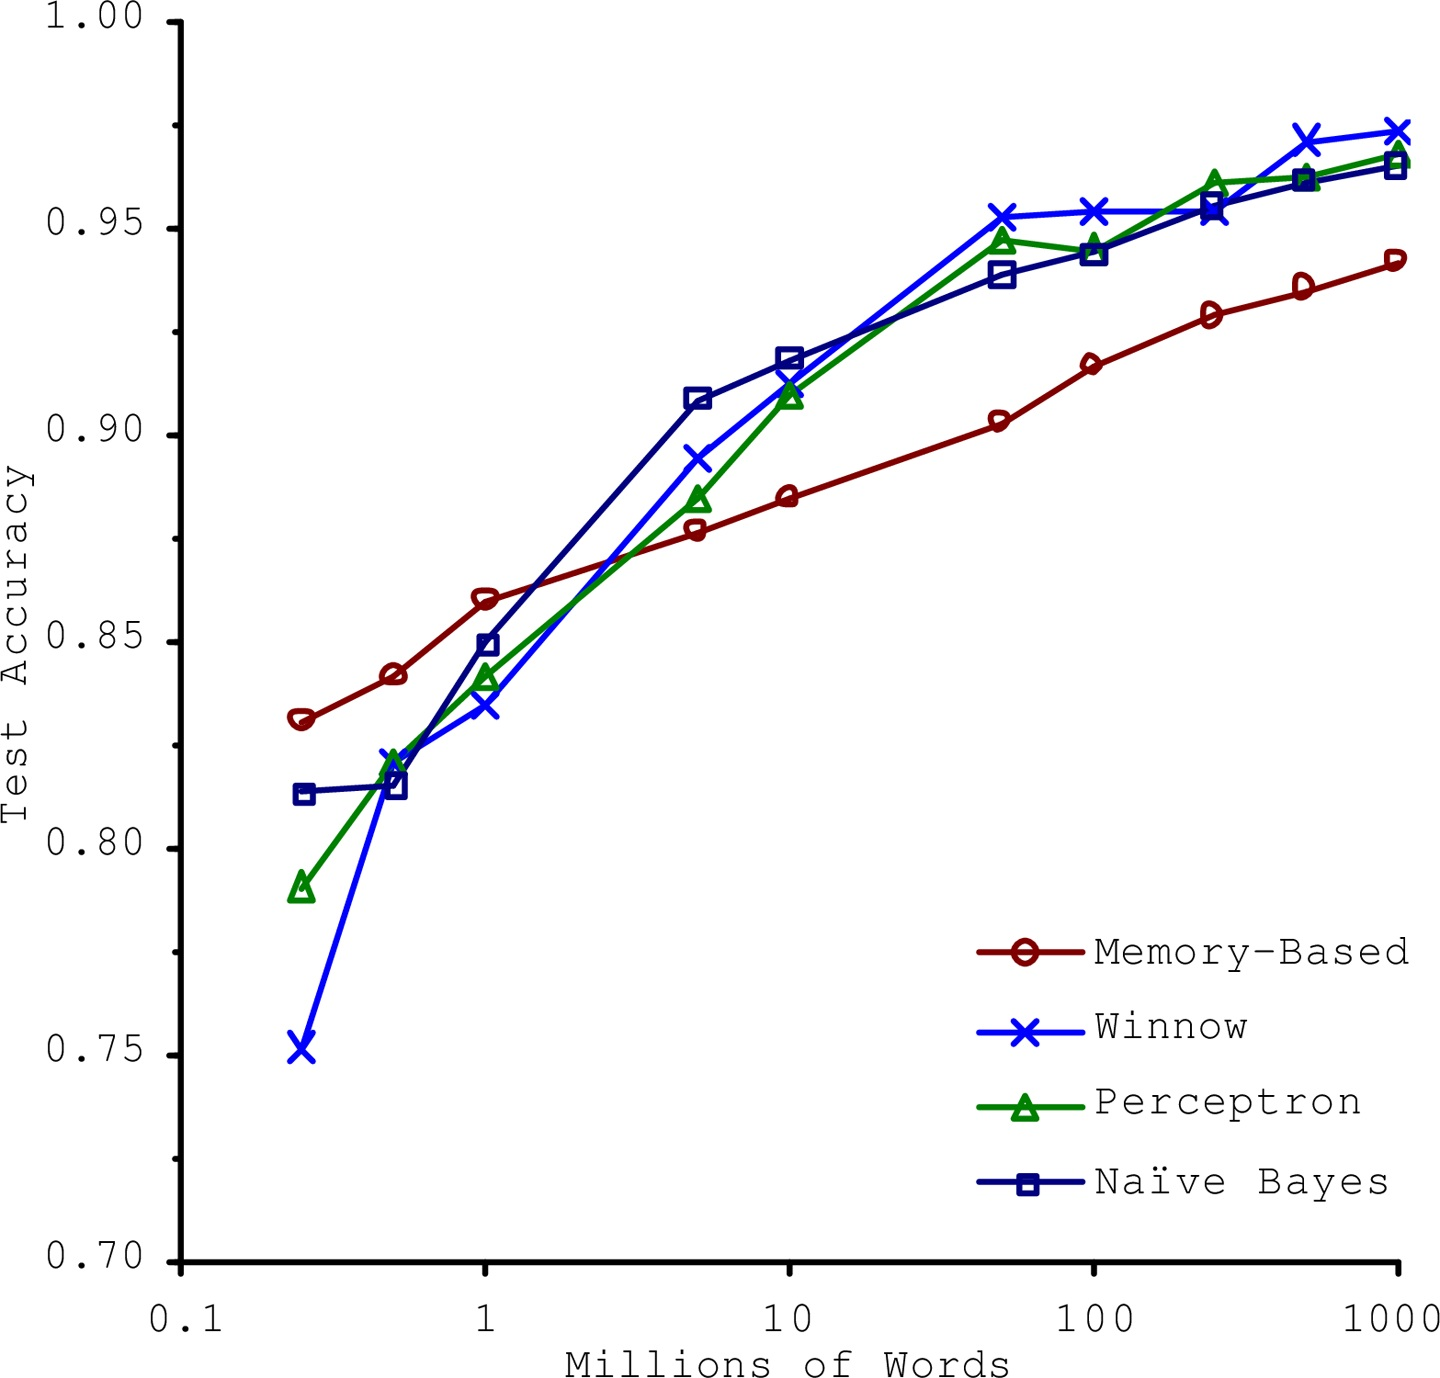
\includegraphics[width=7cm, height=7cm, keepaspectratio]{images/osztalyozas_11.png}
\end{center}
\end{column}
\end{columns}
\end{frame}

\section{Osztályozás}

\begin{frame}
\tableofcontents[currentsection]
\end{frame}

\begin{frame}{Osztályozás}
\begin{columns}
\begin{column}{.5\textwidth}
\begin{block}{Osztályozás}
Az osztályozás a felügyelt gépi tanulás egyik alapvető feladata, amelynek célja, hogy megtanuljon egy modellt vagy szabályrendszert egy adott bemeneti adat alapján \textbf{annak besorolására előre meghatározott kategóriákba vagy csoportokba}. 
\end{block}
\end{column}
\begin{column}{.5\textwidth}
\begin{center}
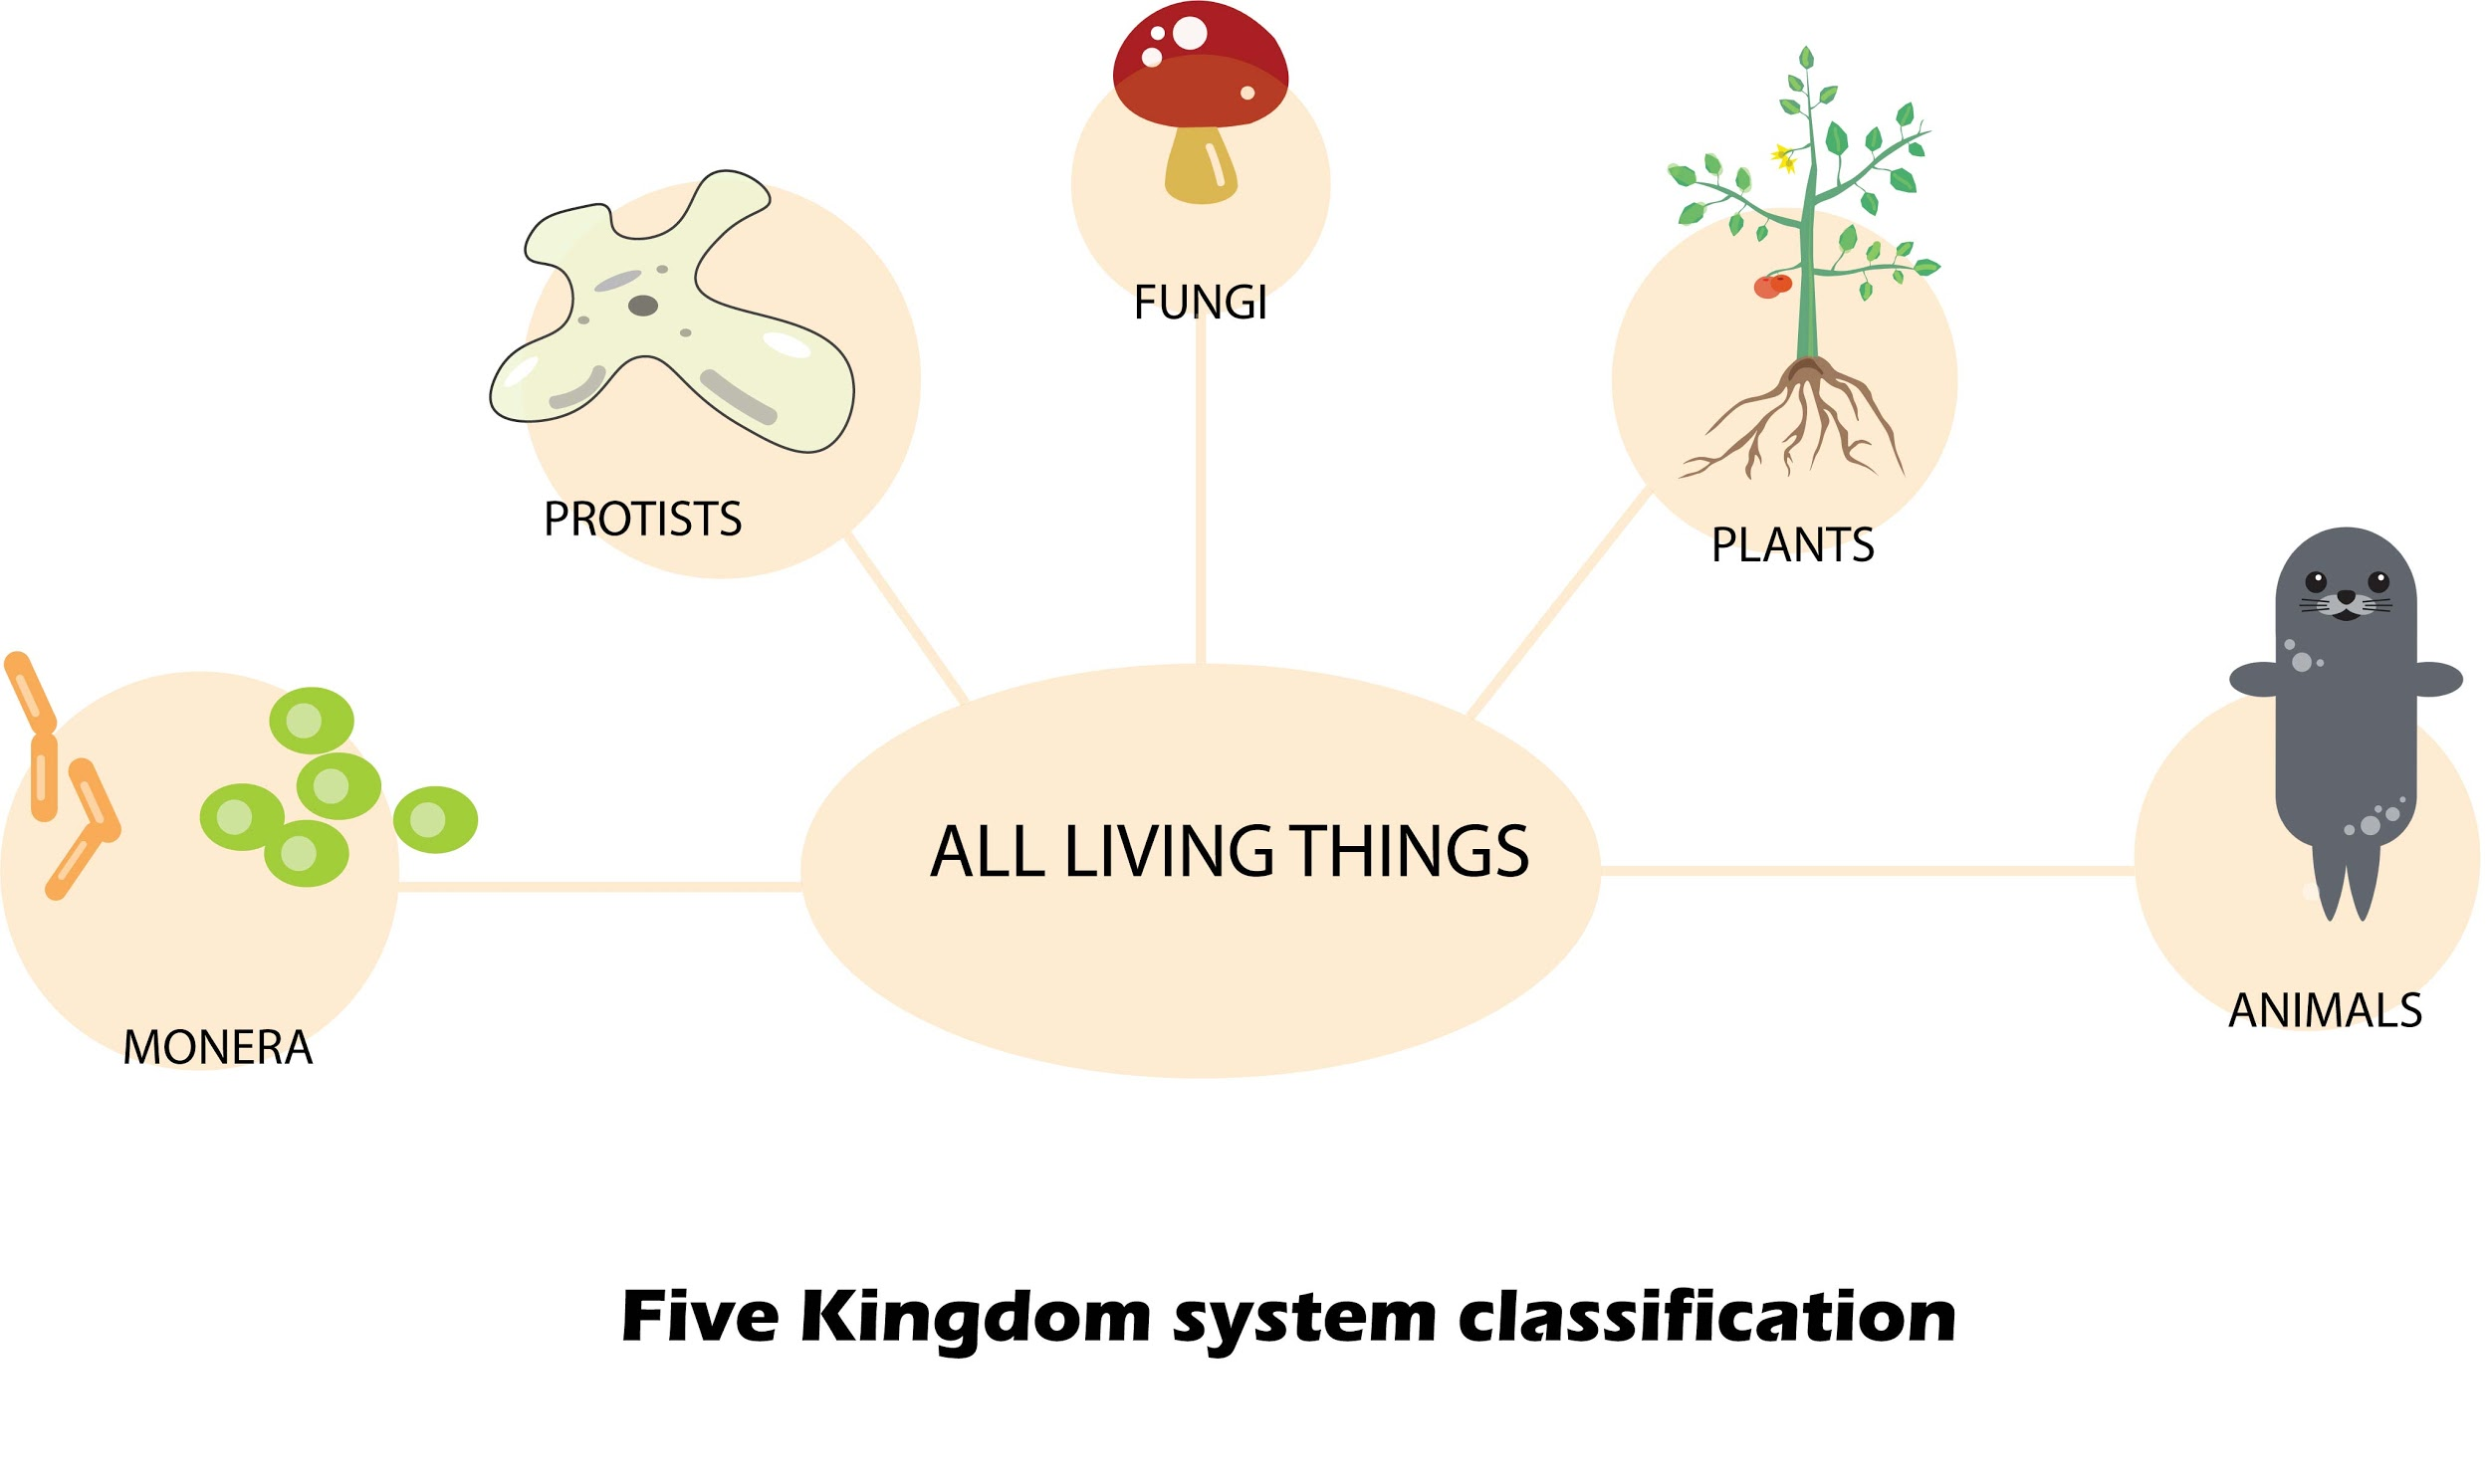
\includegraphics[width=7cm, height=7cm, keepaspectratio]{images/osztalyozas_4.png}
\end{center}
\end{column}
\end{columns}
\end{frame}

\begin{frame}{Modellalapú osztályozás}
\begin{columns}
\begin{column}{.5\textwidth}
Az osztályozó modell feladata, hogy a tanító adathalmaza alapján olyan szabályrendszert hozzon létre, ami \textbf{képes elszeparálni egymástól az egyedeket}.\par\medskip
Amennyiben érkezik egy új adatpont, a modell a saját szabályrendszere segítségével már \textbf{képes lesz becslést adni annak osztályára vonatkozóan}. 
\end{column}
\begin{column}{.5\textwidth}
\begin{center}
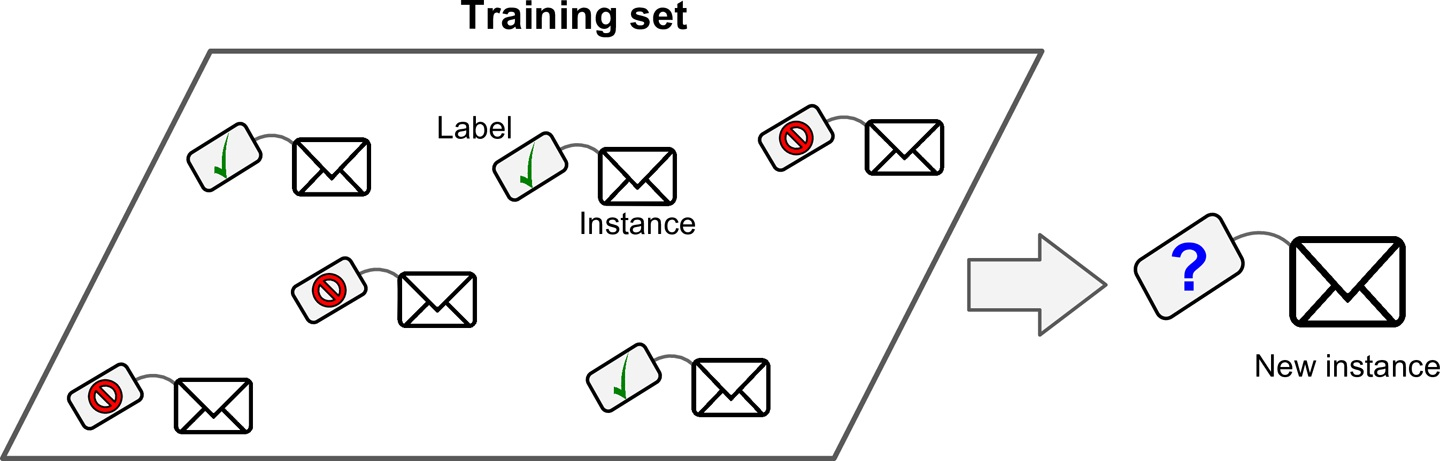
\includegraphics[width=7cm, height=7cm, keepaspectratio]{images/osztalyozas_5.png}
\end{center}
\end{column}
\end{columns}
\end{frame}

\begin{frame}{Modellalapú osztályozás}
\begin{columns}
\begin{column}{.5\textwidth}
\begin{block}{Döntési határ}
Olyan \textbf{határérték, amelyet a modell állít be} az adatpontok különböző osztályokba való besorolásához.\par\smallskip
A határ \textbf{lehet egy vonal, egy sík vagy akár egy sokdimenziós felület}, attól függően, hogy milyen típusú osztályozó modellt használunk és milyen a bemeneti adatok dimenzionalitása.
\end{block}
\end{column}
\begin{column}{.5\textwidth}
\begin{center}
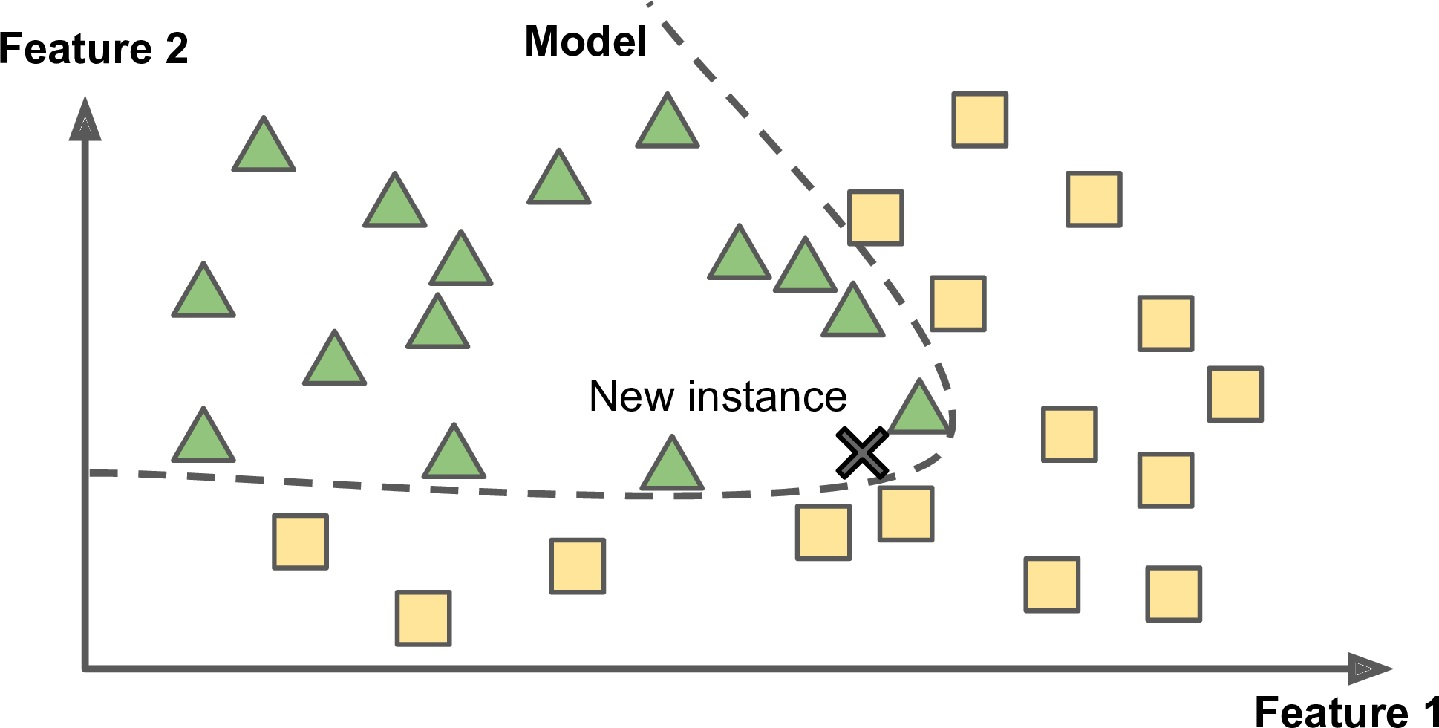
\includegraphics[width=7cm, height=7cm, keepaspectratio]{images/osztalyozas_6.png}
\end{center}
\end{column}
\end{columns}
\end{frame}

\begin{frame}{Az osztályozás fajtái}
\begin{columns}
\begin{column}{.5\textwidth}
\only<1>{\begin{block}{Bináris osztályozás}
A modell két lehetséges osztály közül valamelyikbe sorolja be az egyedeket. Minden egyedhez csakis 1 osztály tartozhat.
\end{block}}
\only<2>{\begin{block}{Multiosztályos osztályozás}
Több, mint két lehetséges kategória létezik, amibe az egyedek besorolhatók, ezek közül az egyikbe fog sorolódni az egyed. Minden egyedhez legalább és legfeljebb 1 osztály tartozik.
\end{block}}
\only<3>{\begin{block}{Multicímkés osztályozás}
Minden mintaegyedhez több bináris vagy multicímkés címkekategóriából tartozhat osztály.
\end{block}}
\only<4>{\begin{block}{Multioutput osztályozás}
A multicímkés osztályozás generalizált változata. Egy egyedhez egy multicímkés halmazból több elem is tartozhat.
\end{block}}
\end{column}
\begin{column}{.5\textwidth}
\only<1>{\begin{center}
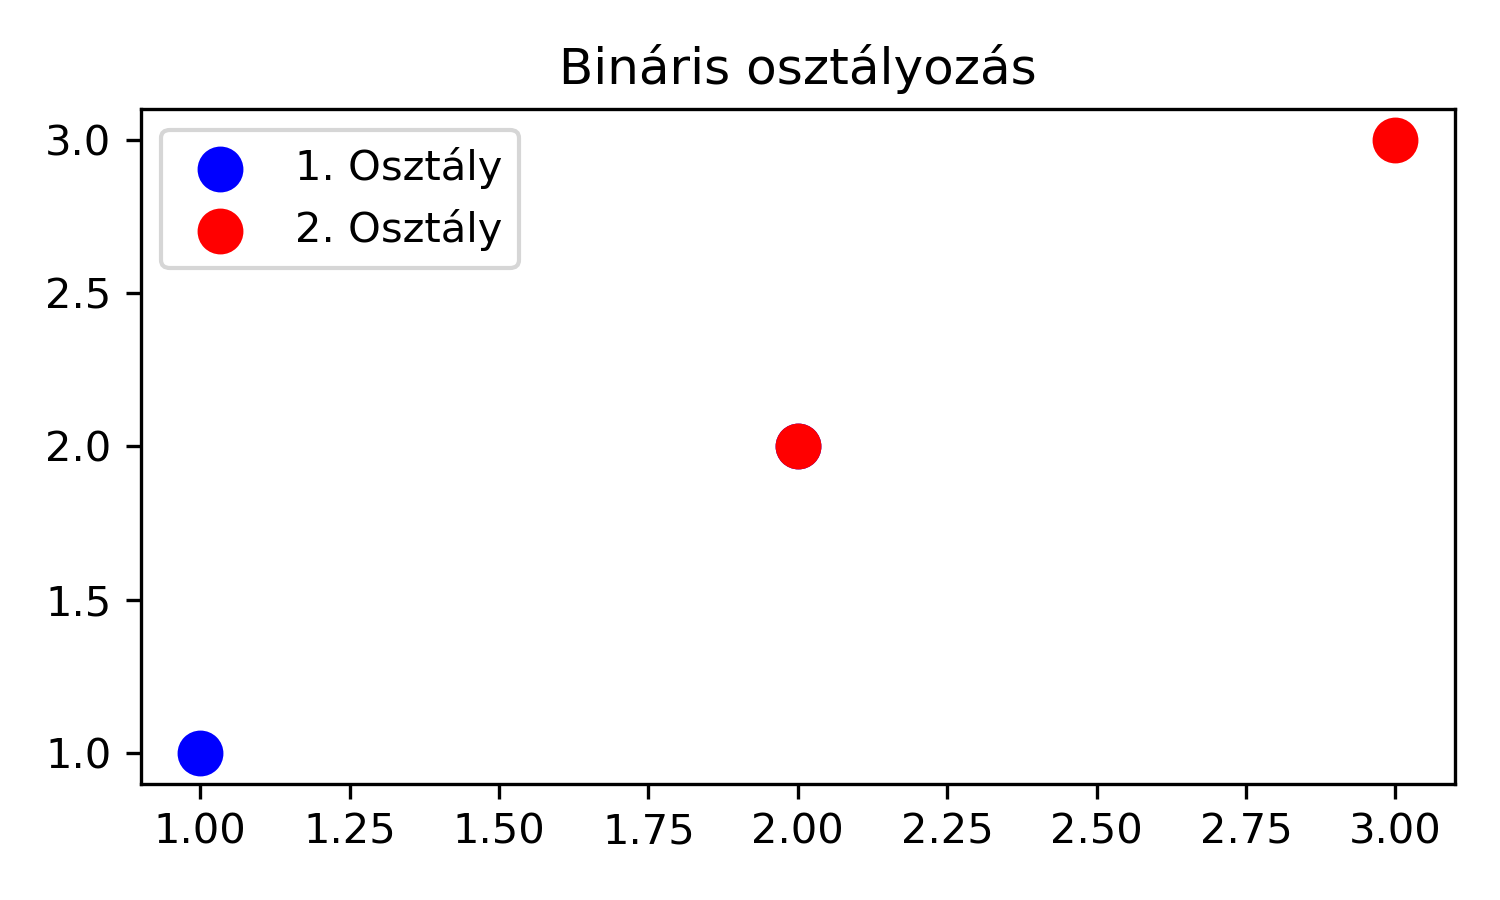
\includegraphics[width=7cm, height=7cm, keepaspectratio]{images/osztalyozas_7.png}
\end{center}}
\only<2>{\begin{center}
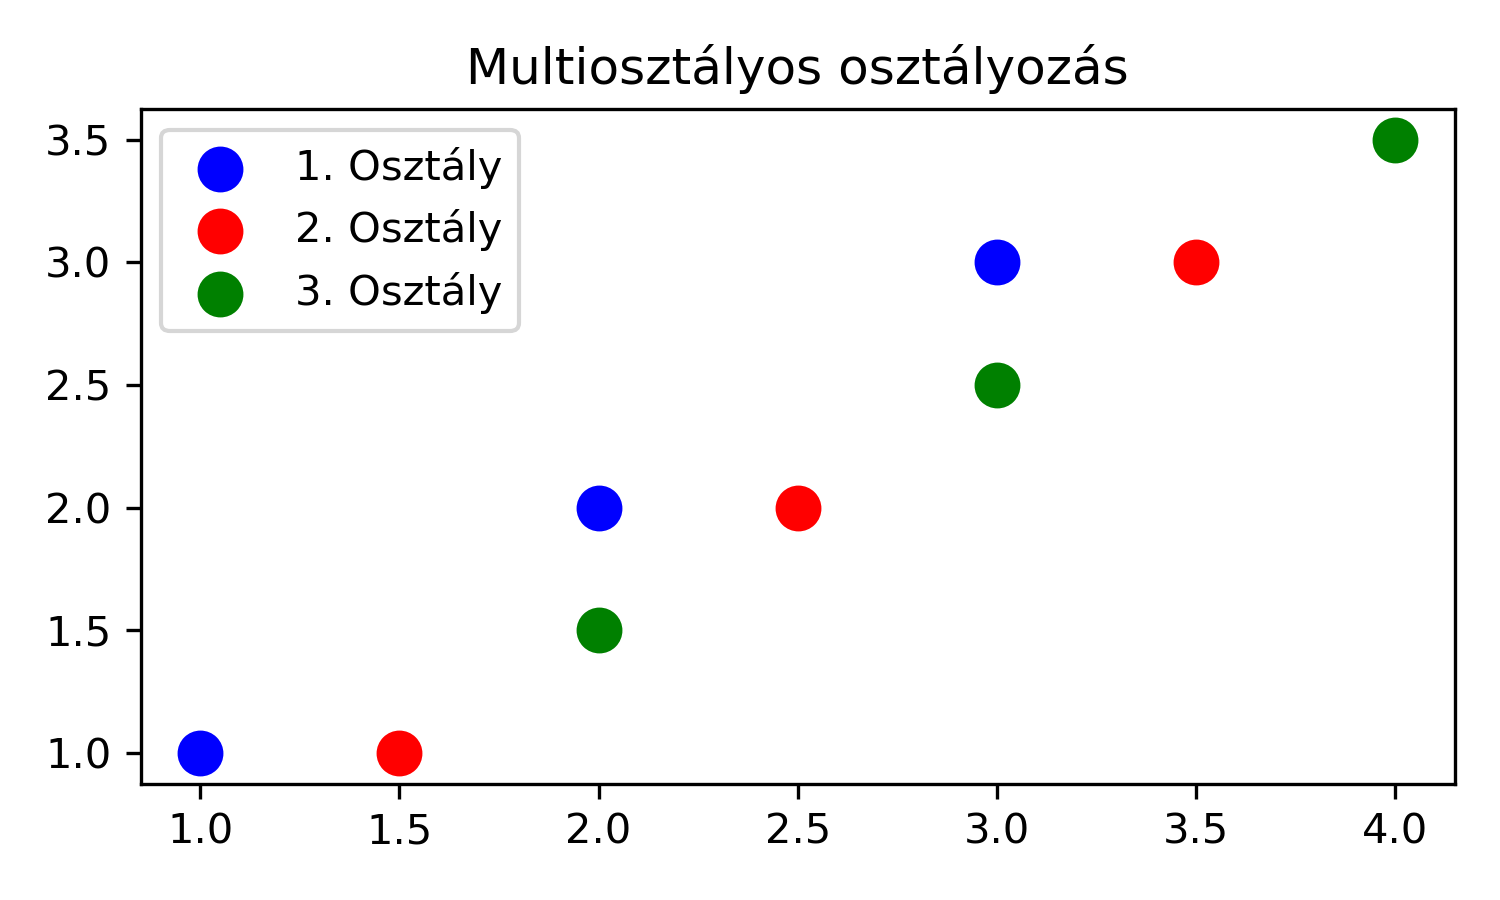
\includegraphics[width=7cm, height=7cm, keepaspectratio]{images/osztalyozas_8.png}
\end{center}}
\only<3>{\begin{center}
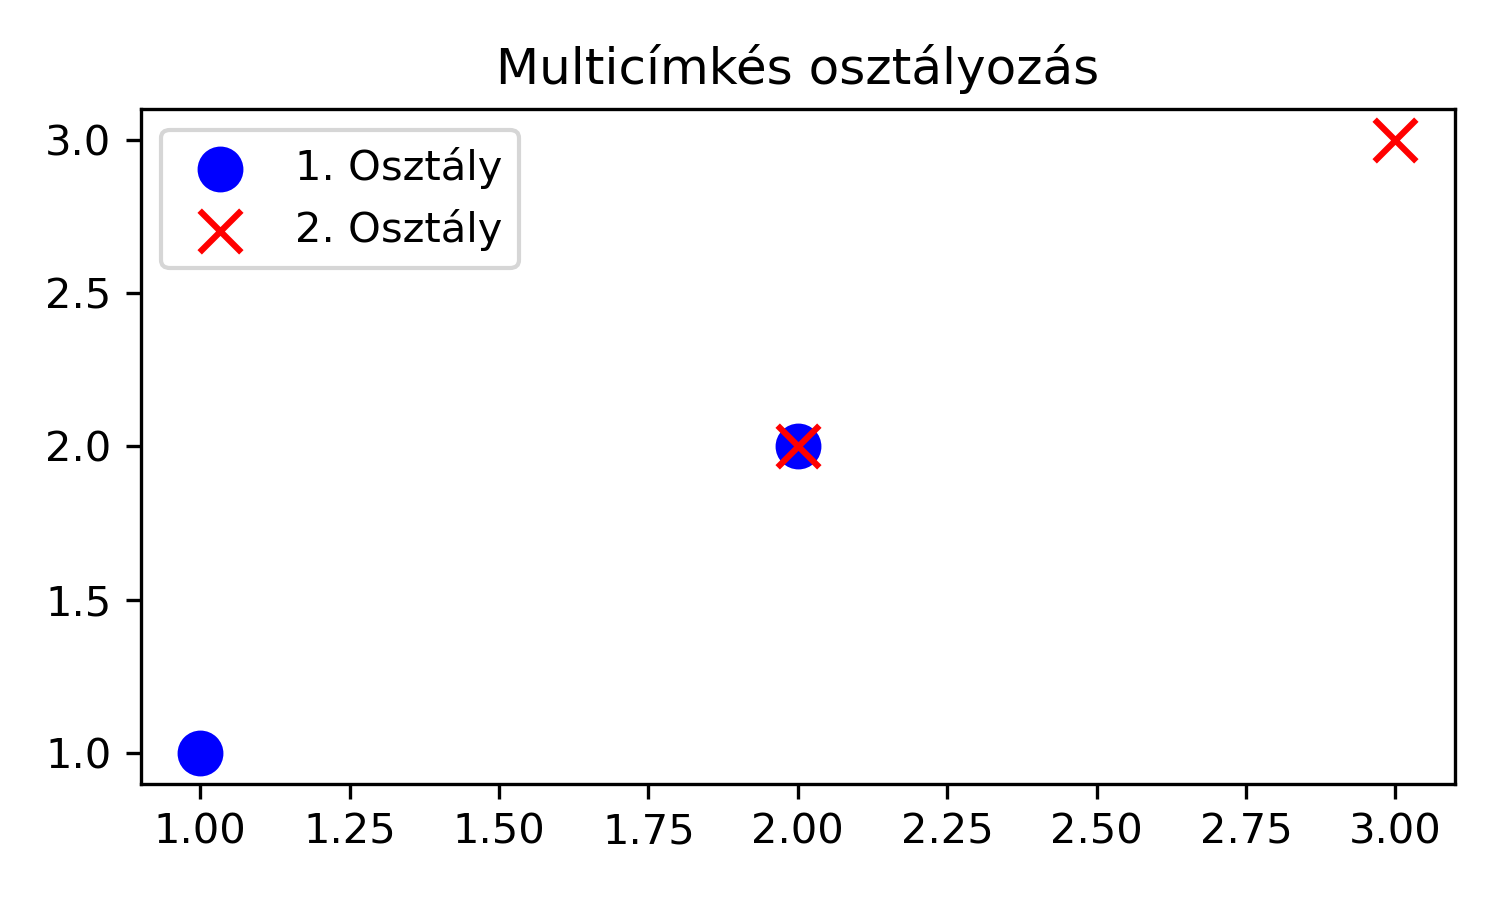
\includegraphics[width=7cm, height=7cm, keepaspectratio]{images/osztalyozas_9.png}
\end{center}}
\only<4>{\begin{center}
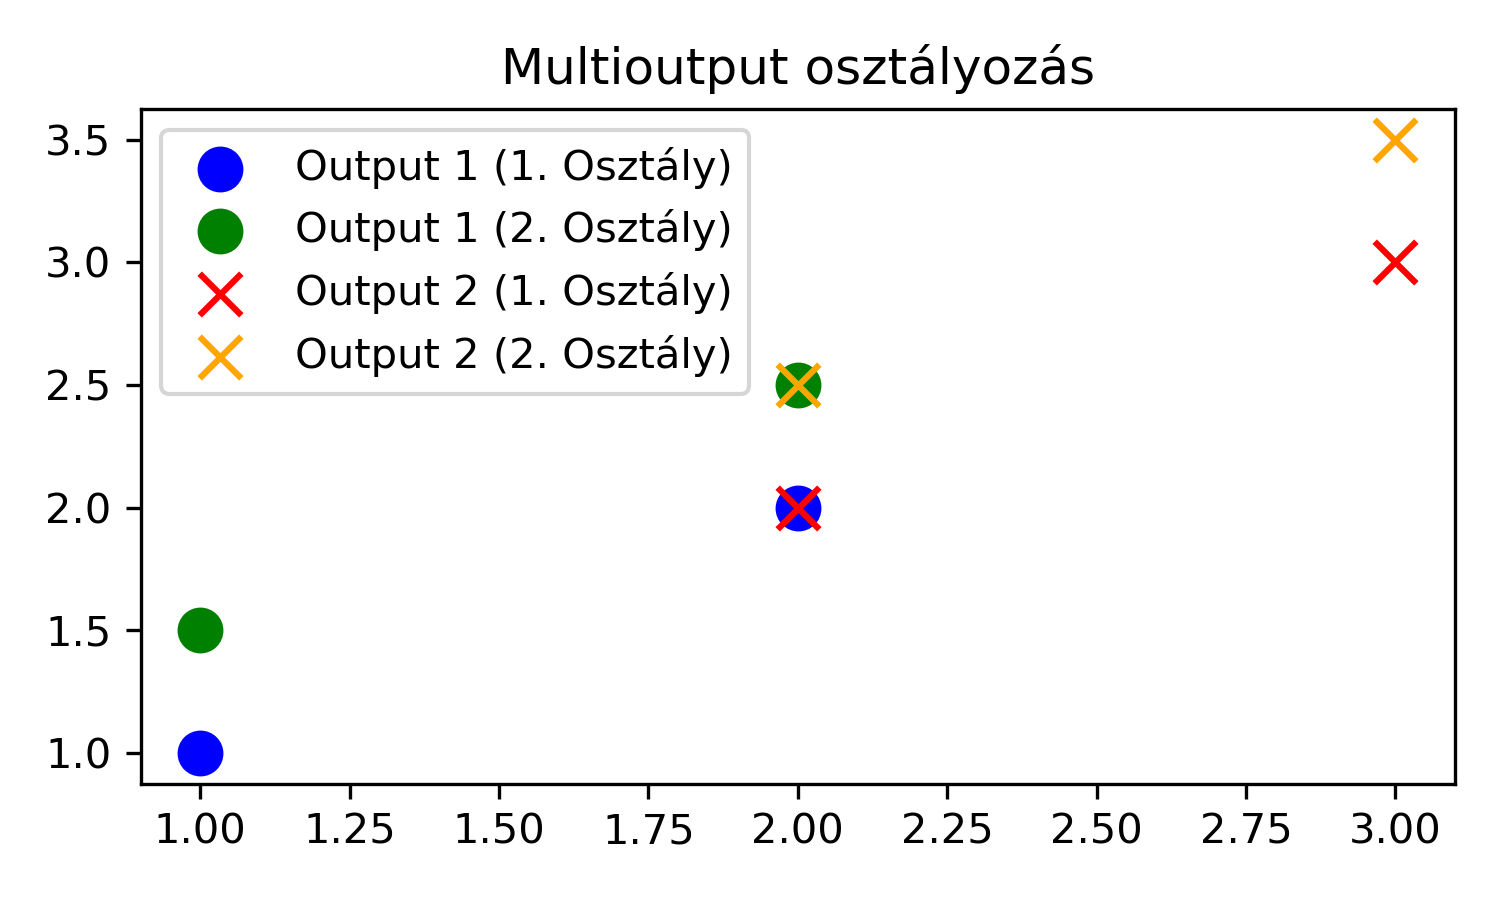
\includegraphics[width=7cm, height=7cm, keepaspectratio]{images/osztalyozas_10.png}
\end{center}}
\end{column}
\end{columns}
\end{frame}

\section{Osztályozás vagy regresszió?}

\begin{frame}
\tableofcontents[currentsection]
\end{frame}

\begin{frame}{Példa: a probléma bemutatása}
\begin{columns}
\begin{column}{.5\textwidth}
A következő kis adathalmaz három sakkjátszmának rögzítette az eredményét. Minden meccs esetén rögzítésre kerültek a következő rekordok:\par\medskip
\begin{center}
\begin{tabular}{|c|c|}
\hline
Különbség & Nyertes\\
\hline
$200$ & $0$\\
\hline
$-200$ & $1$\\
\hline
$300$ & $0$\\
\hline
\end{tabular}
\end{center}
\end{column}
\begin{column}{.5\textwidth}
Ebben az esetben az $x$ változó, a \textbf{két játékos rangjának különbsége} a fehér és fekete játékos különbségét jelzi, az $y$ célváltozó pedig egy azt a valószínűséget jelenti, hogy \textbf{a fehér nyert-e}.
\begin{center}
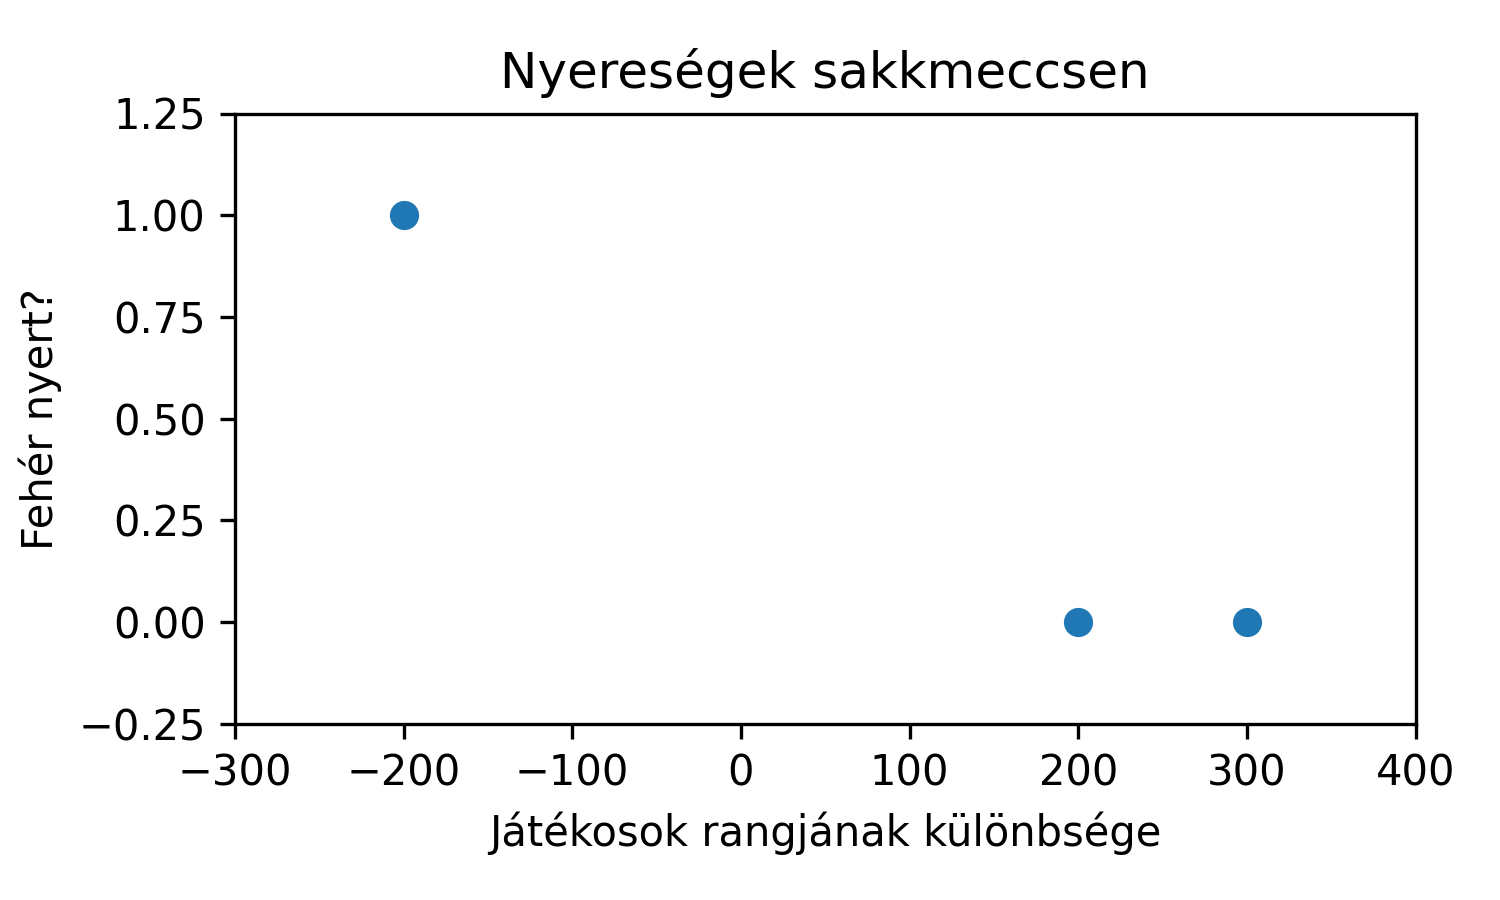
\includegraphics[width=7cm, height=7cm, keepaspectratio]{images/osztalyozas_12.png}
\end{center}
\end{column}
\end{columns}
\end{frame}

\begin{frame}{Példa: lineáris predikció}
\begin{columns}
\begin{column}{.5\textwidth}
Az adathalmazra egy lineáris regresszor modellt illesztve az eredmény a következő:\par\smallskip
\begin{center}
\begin{tabular}{|c|c|c|}
\hline
Különbség & Nyertes & Predikció\\
\hline
$200$ & $0$ & $0.11$\\
\hline
$-200$ & $1$ & $0.97$\\
\hline
$300$ & $0$ & $-0.1$\\
\hline
\end{tabular}
\par\medskip
\end{center}
Ebben az estben a lineáris modell:
\begin{block}{}
\vspace{-0.6cm}
\[
\hat{y} = \theta_0 + \theta_1 \cdot x = 0.54 - 0.0021 \cdot x
\]
\end{block}
Ahol $\hat{y}$ a modell predikciója a nyertesre vonatkozóan, $\theta_0$ a konstans torzítás, $\theta_1$ a függvény meredeksége és $x$ a két játékos rangjának különbsége.
\end{column}
\begin{column}{.5\textwidth}
Az adatpontokra egy lineáris regressziós függvényt illesztve az illesztett modell a következő lesz:\par\smallskip
\begin{center}
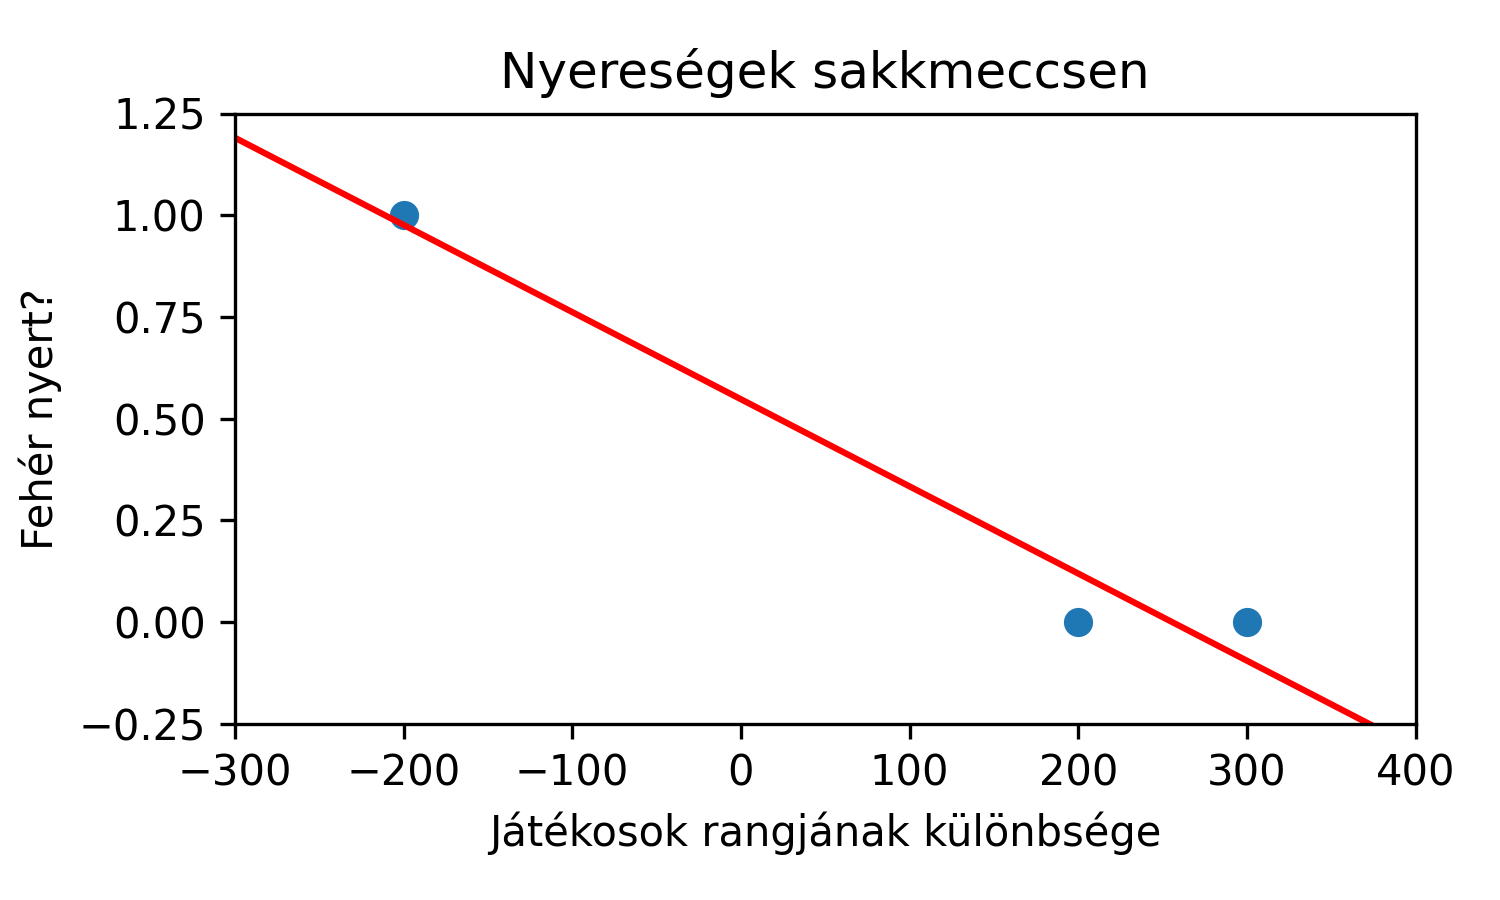
\includegraphics[width=7cm, height=7cm, keepaspectratio]{images/osztalyozas_13.png}
\end{center}
\end{column}
\end{columns}
\end{frame}

\begin{frame}{Példa: következtetések}
\begin{columns}
\begin{column}{.5\textwidth}
A lineáris modell nem minden esetben ad racionális predikciót az adathalmazra vonatkozóan.\par\smallskip
\textbf{Negatív valószínűségek nem értelmezettek!}\par\smallskip
Éppen ezért ha a modellezés célváltozója egy valószínűség, szükség van arra, hogy az illesztett modell szélsőértéke $0$ legyen ha a hely $-\infty$ és $1$ ha a hely $\infty$.
\end{column}
\begin{column}{.5\textwidth}
\begin{center}
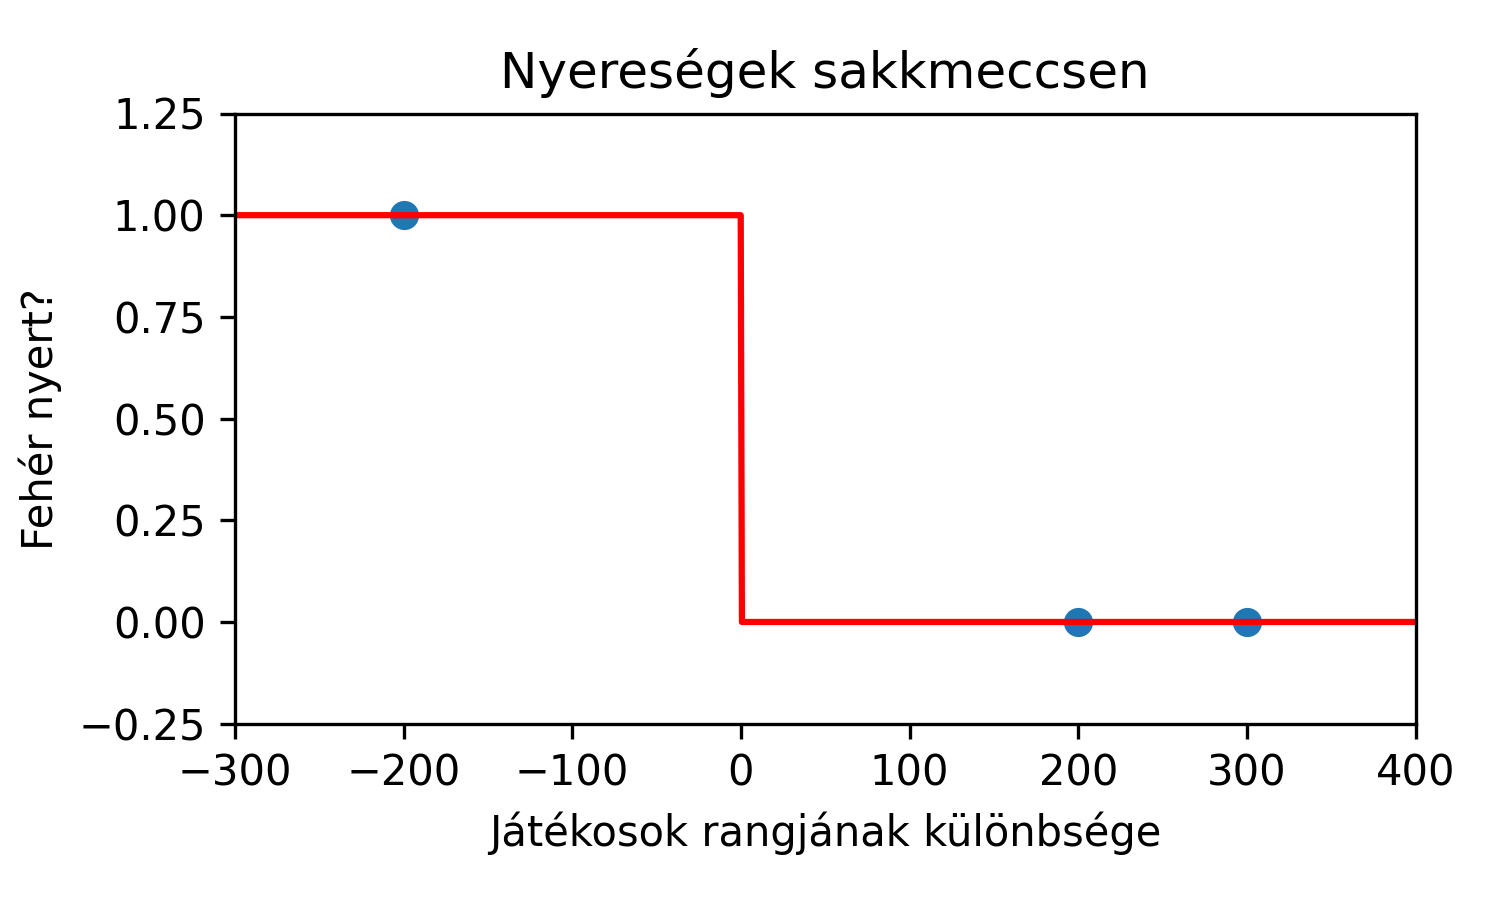
\includegraphics[width=7cm, height=7cm, keepaspectratio]{images/osztalyozas_14.png}
\end{center}
\end{column}
\end{columns}
\end{frame}

\section{Osztályozás jósága}

\begin{frame}
\tableofcontents[currentsection]
\end{frame}

\begin{frame}{Az osztályozás teljesítményének mérése}
\begin{columns}
\begin{column}{.5\textwidth}
\only<1>{\begin{itemize}
	\item \textbf{Valós pozitív (TP)}: Pozitív egyed, és annak is van osztályozva
	\item \textbf{Valós negatív (TN)}: Negatív egyed, és annak is van osztályozva
	\item \textbf{Hamis pozitív (FP)}: Negatív egyed, de pozitívnak van osztályozva
	\item \textbf{Hamis negatív (FN)}: Pozitív egyed, de negatívnak van osztályozva
\end{itemize}}
Ennek alapján két fő mutatószám áll elő, amellyel egy osztályozó modellt lehetséges értékelni:
\only<2>{
\begin{block}{Pontosság}
Megadja, hogy a pozitívnak osztályozott egyedek közül mekkora hányad volt ténylegesen pozitív:
\[
P = \frac{TP}{TP+FP}
\]
\end{block}}
\only<3>{
\begin{block}{Visszahívás}
Megadja, hogy az összes pozitív egyed mekkora hányadát osztályozta a modell pozitívnak:
\[
R = \frac{TP}{TP + FN}
\]
\end{block}}
\end{column}
\begin{column}{.5\textwidth}
\begin{center}
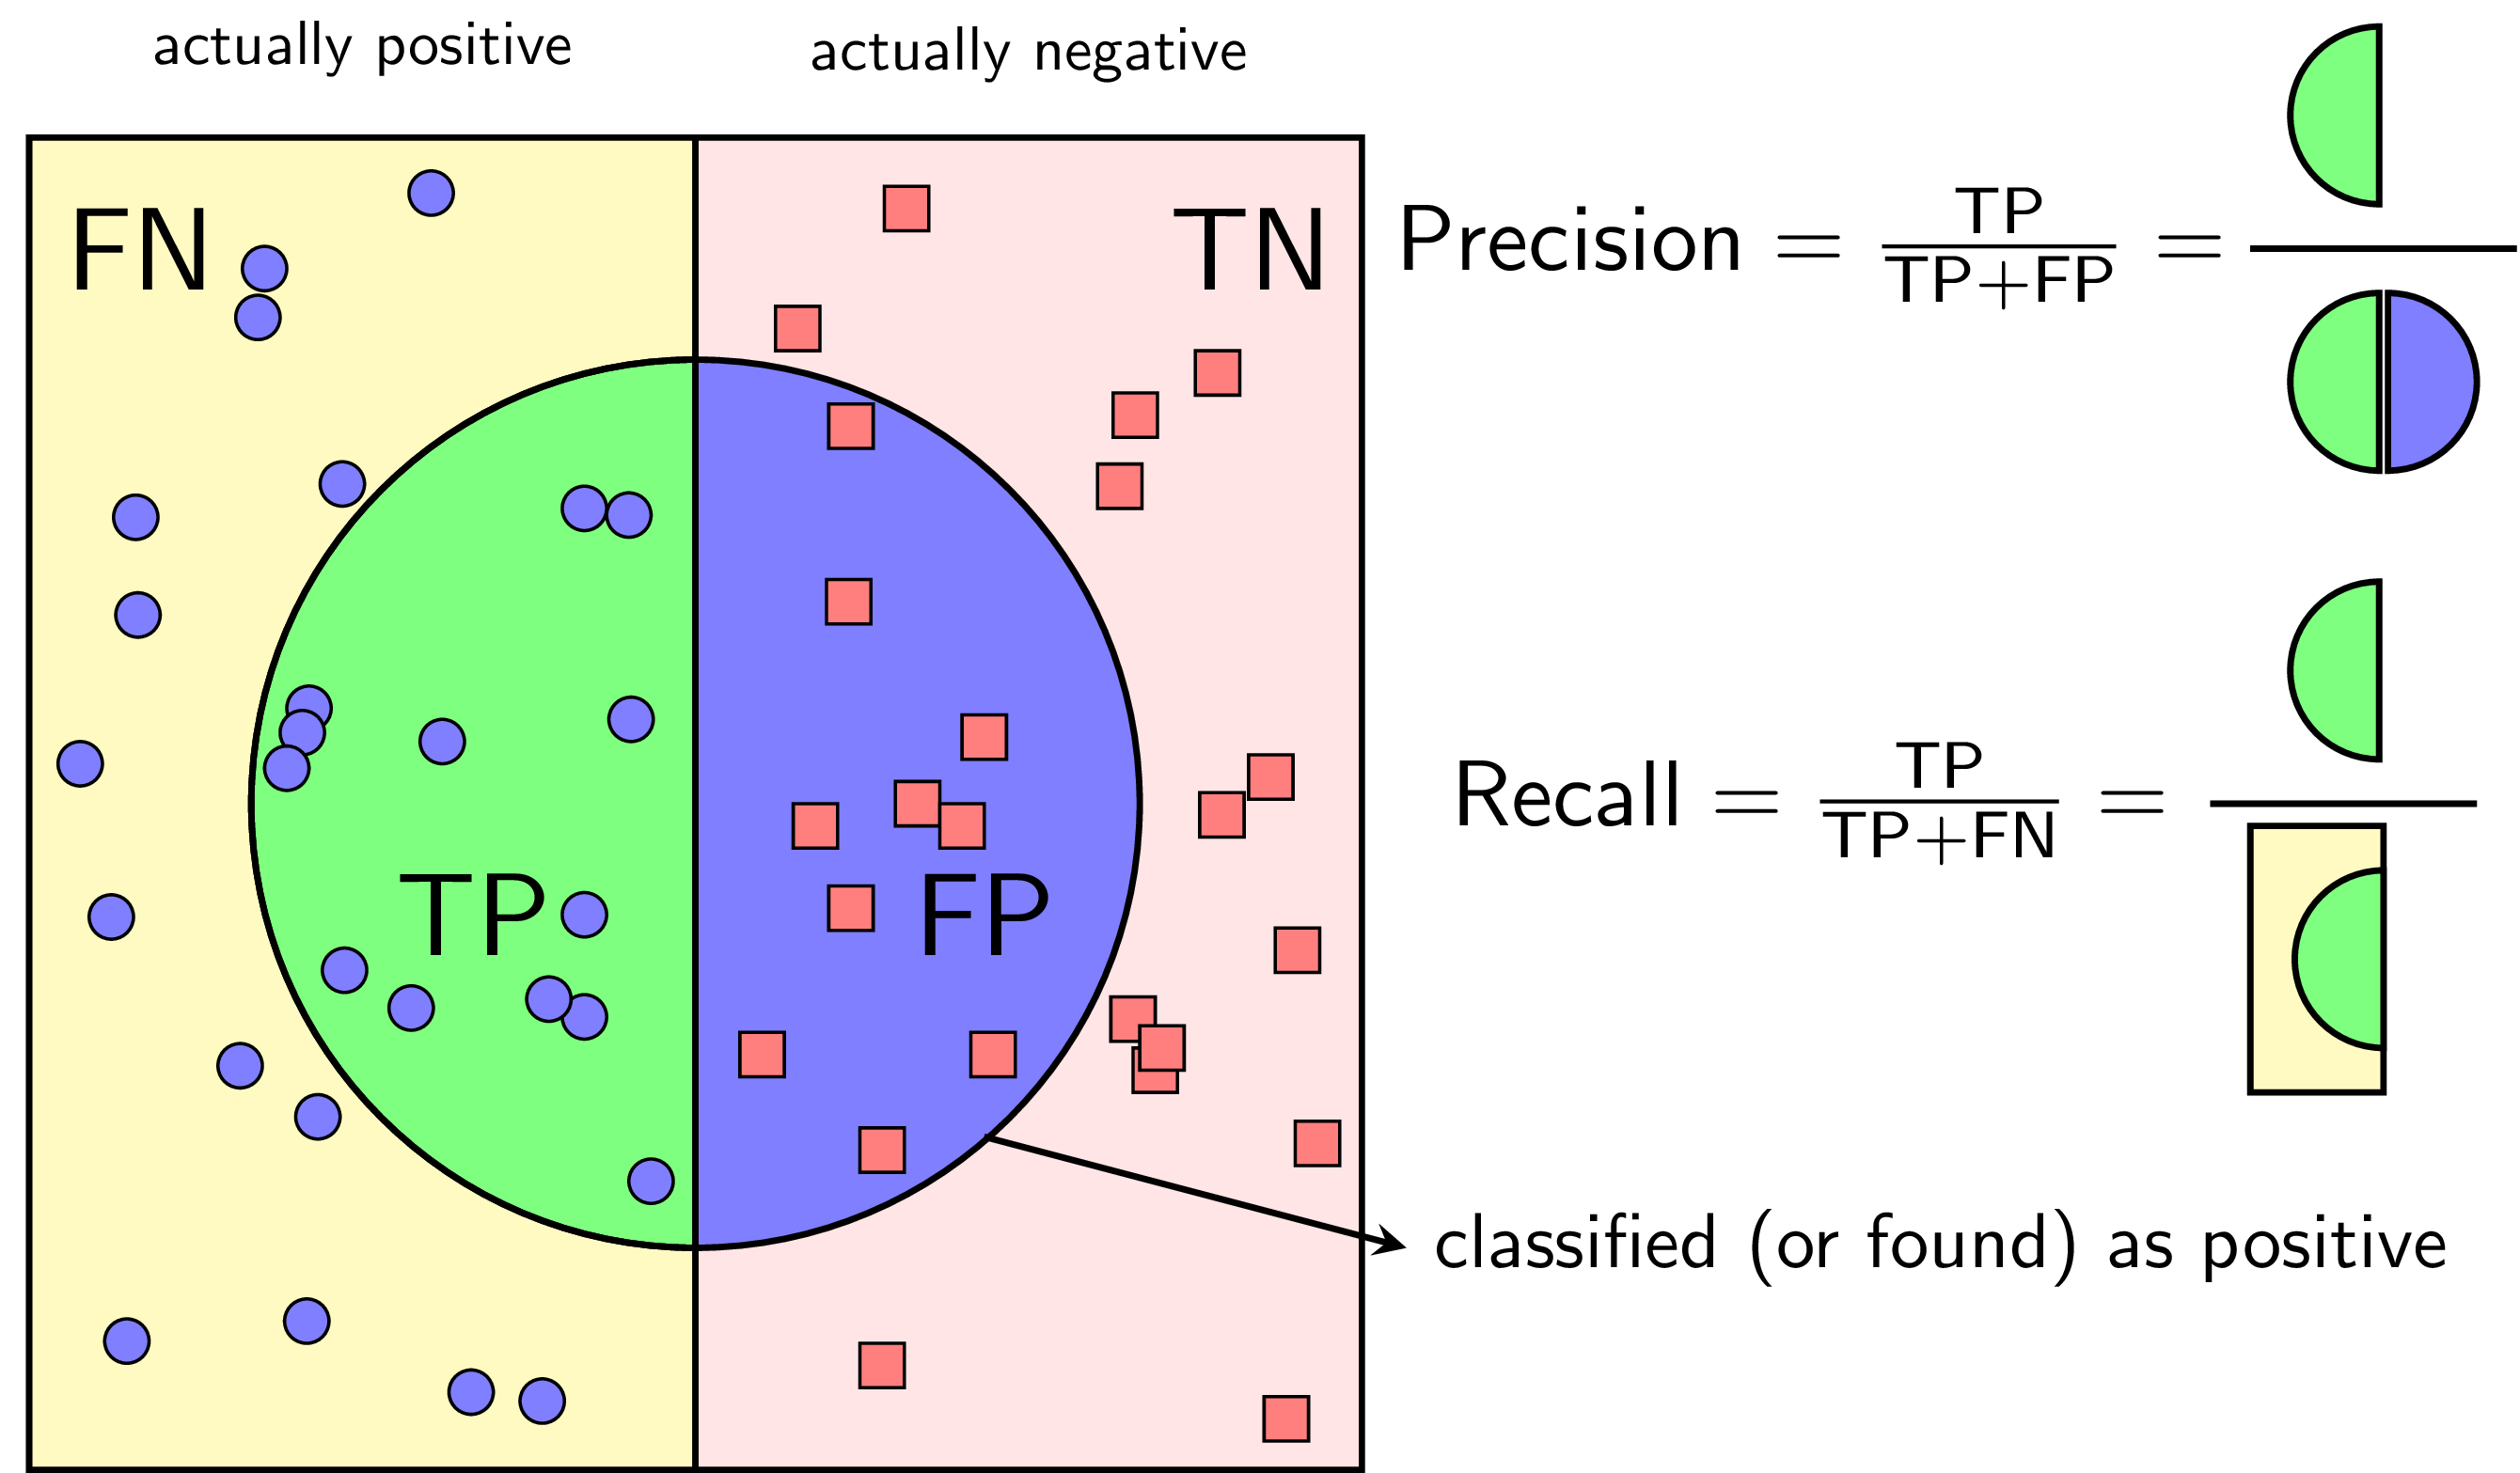
\includegraphics[width=7cm, height=7cm, keepaspectratio]{images/osztalyozas_15.png}
\end{center}
\end{column}
\end{columns}
\end{frame}

\begin{frame}{Konfúziós mátrix}
\begin{columns}
\begin{column}{.5\textwidth}
A konfúziós mátrix vagy zavarmátrix a statisztikában és gépi tanulásban használatos egy gépi tanulási \textbf{algoritmus teljesítményének mérésére}.\par\smallskip
A mátrix segít megérteni, hogy \textbf{milyen hibákat követett el a modell} és ezáltal segíti a modell finomhangolását és tovább tanítását.\par\smallskip
A mátrix általánosítható tetszőleges címke számra. 
\end{column}
\begin{column}{.5\textwidth}
\begin{center}
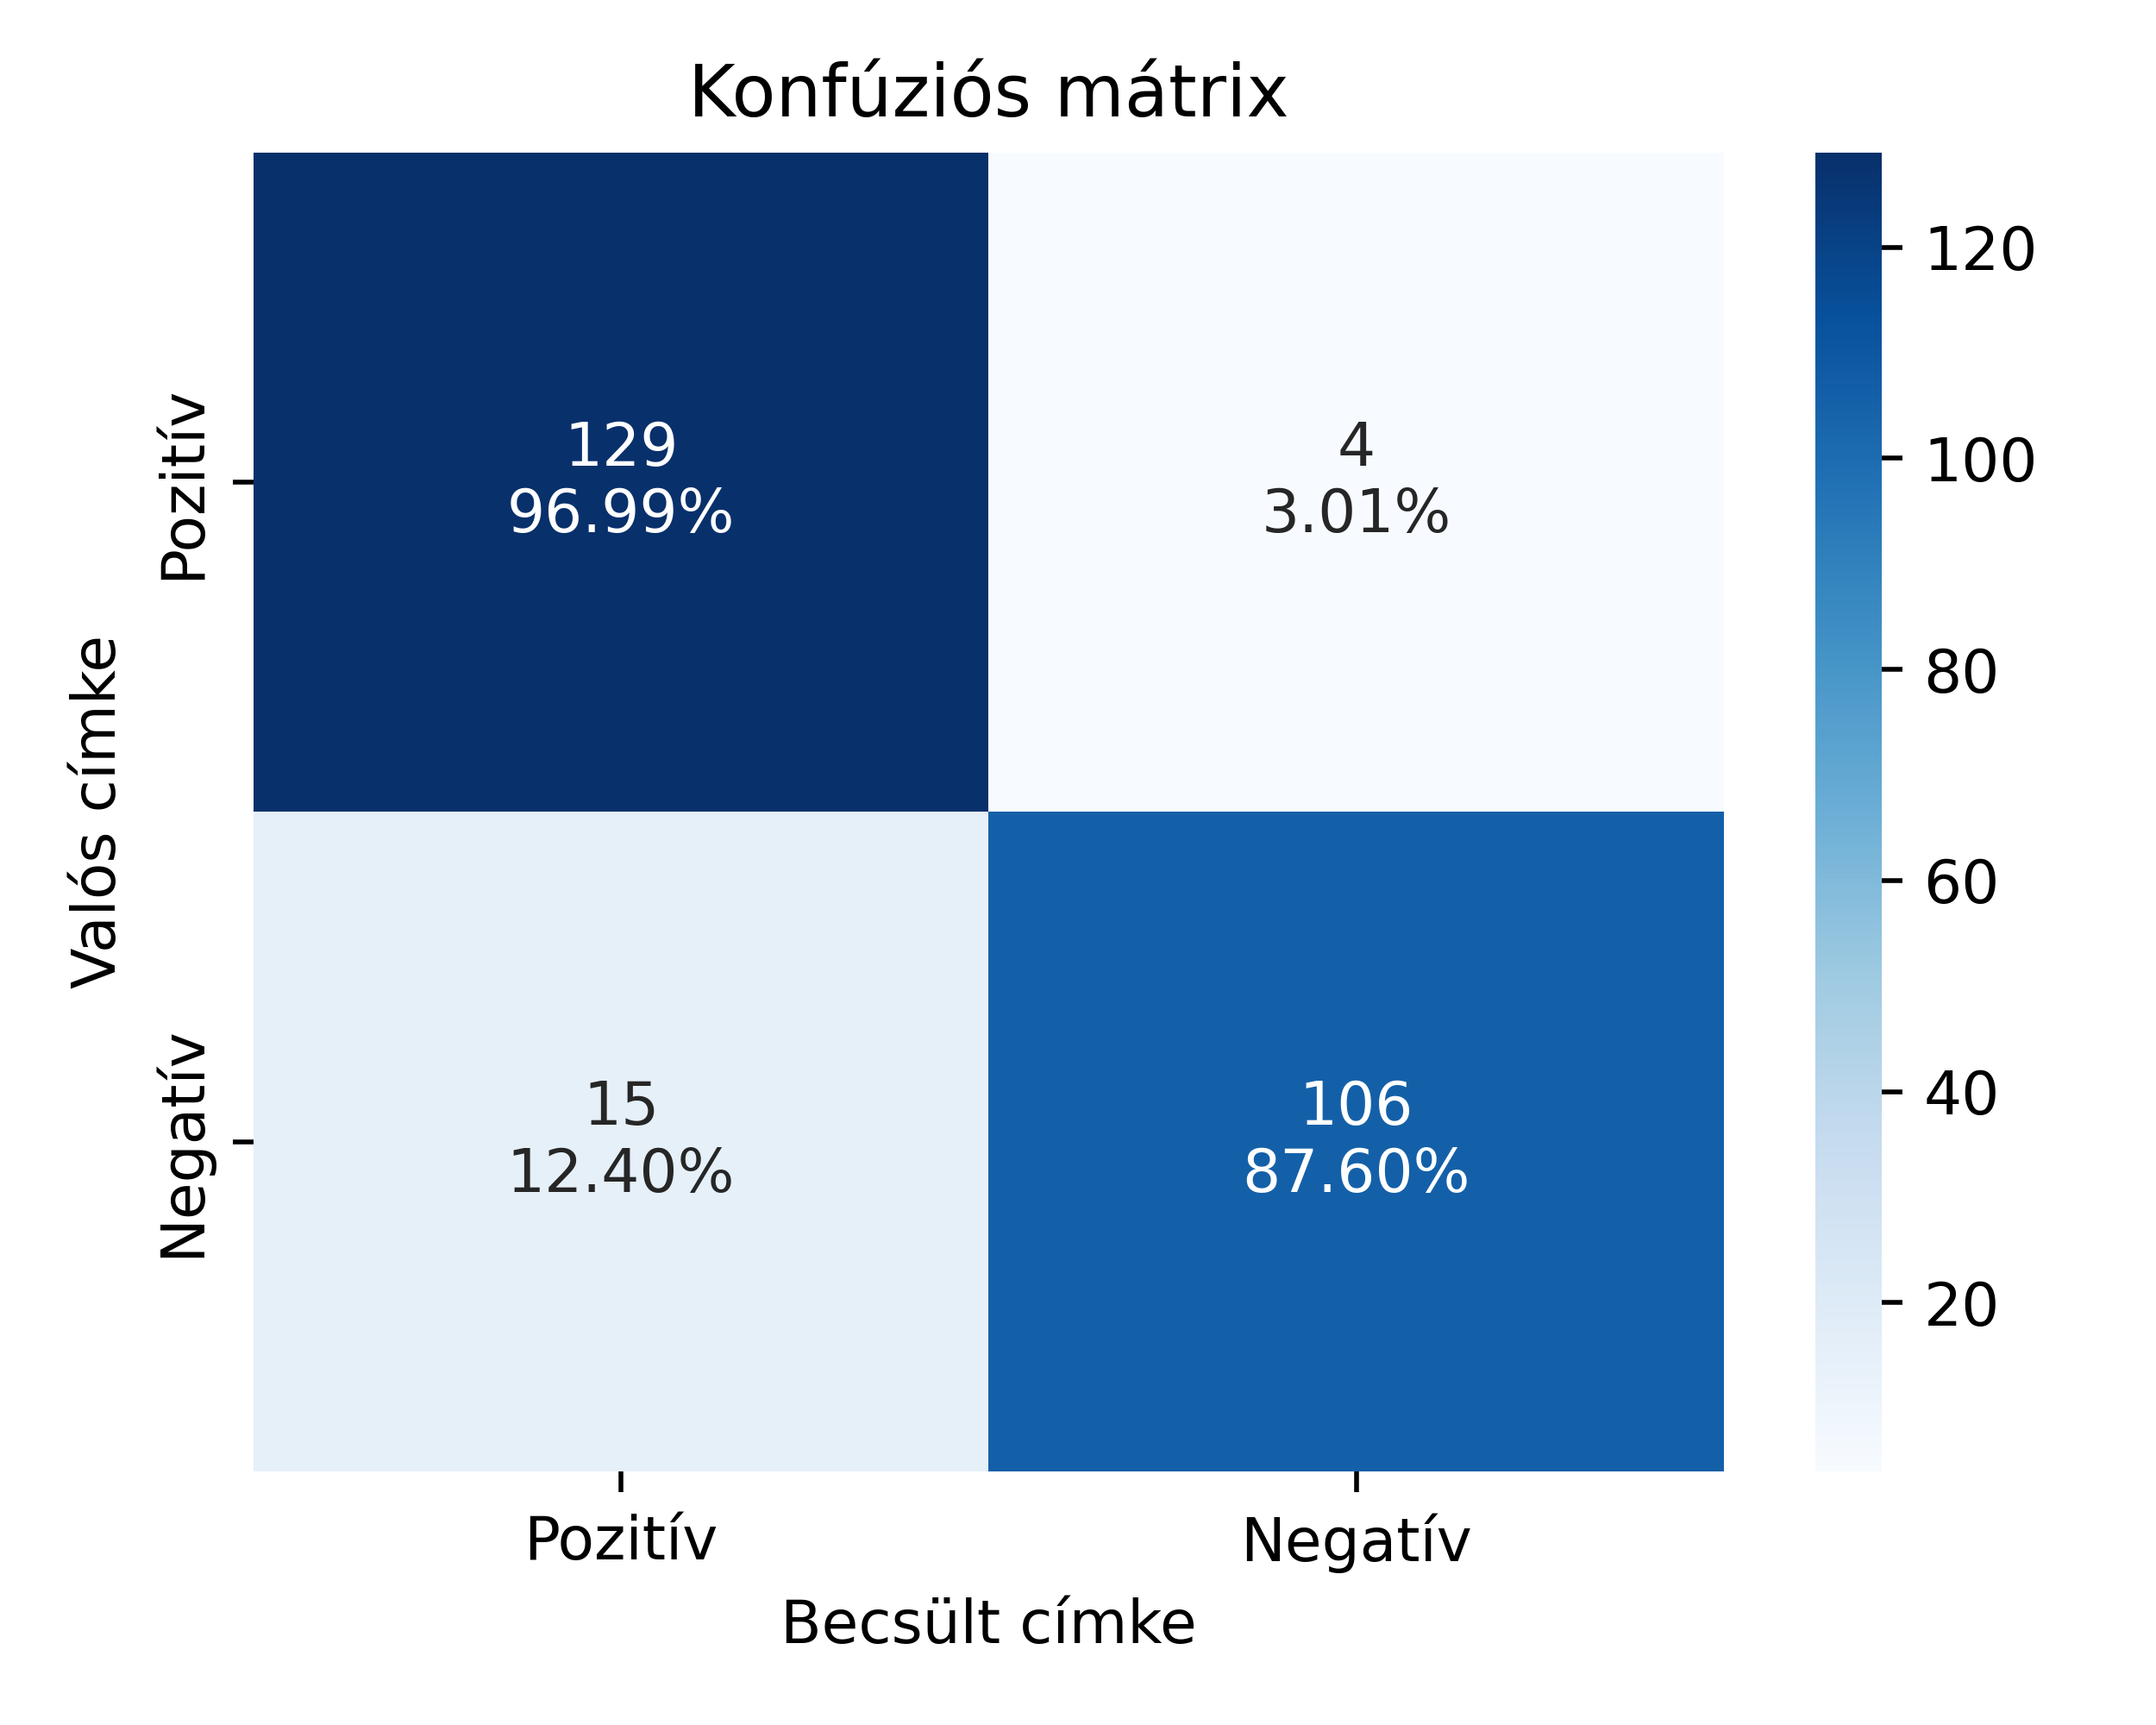
\includegraphics[width=7cm, height=6cm, keepaspectratio]{images/osztalyozas_17.png}
\end{center}
\end{column}
\end{columns}
\end{frame}

\section{Logisztikus regresszió}

\begin{frame}
\tableofcontents[currentsection]
\end{frame}

\begin{frame}{Logisztikus regresszió}
\begin{columns}
\begin{column}{.5\textwidth}
Gépi tanulási módszer kétosztályos (bináris) kimenetelek előrejelzésére, amely valószínűségek megbecslésére szolgál. A logisztikus regresszió eljárása:\par\smallskip
\begin{enumerate}
	\item Adott mintaegyedre annak a valószínűségnek a megbecslése, hogy a modell a pozitív osztályba tartozik-e. 
	\item Ha a becsült valószínűség magasabb mint egy küszöbérték, a becsült osztály pozitív, egyébként negatív.
\end{enumerate}
\end{column}
\begin{column}{.5\textwidth}
\begin{block}{}
\[
\hat{y}\begin{cases}
_{1}^{0} & _{ha\;\hat{p}\,\leq\,\theta}^{ha\;\hat{p}\,>\,\theta}\end{cases}
\]
Ahol $\hat{p}$ a modell által becsült valószínűség, $\hat{y}$ a becsült osztály és $\theta$ a küszöbérték.
\end{block}
\end{column}
\end{columns}
\end{frame}

\begin{frame}{A logisztikus (szigmoid) függvény}
\begin{columns}
\begin{column}{.5\textwidth}
A logisztikus függvény a valószínűségek megbecslésére használt modell típus. A predikció előállításához először az eljárás előállítja $z$ lineáris predikciót:
\begin{block}{}
\vspace{-.6cm}
\[
z = \theta_0 + \theta_1x_1 + \theta_2x_2 + \ldots + \theta_rx_r
\]
\end{block}
Majd ezt behelyettesíti a logisztikus függvénybe: 
\begin{block}{}
\[
\sigma\left( z \right) = \frac{1}{1 + e^z}
\]
\end{block}
Ahol $\sigma$ a logisztikus függvény és $e$ a természetes logaritmus értéke. 
\end{column}
\begin{column}{.5\textwidth}
\begin{center}
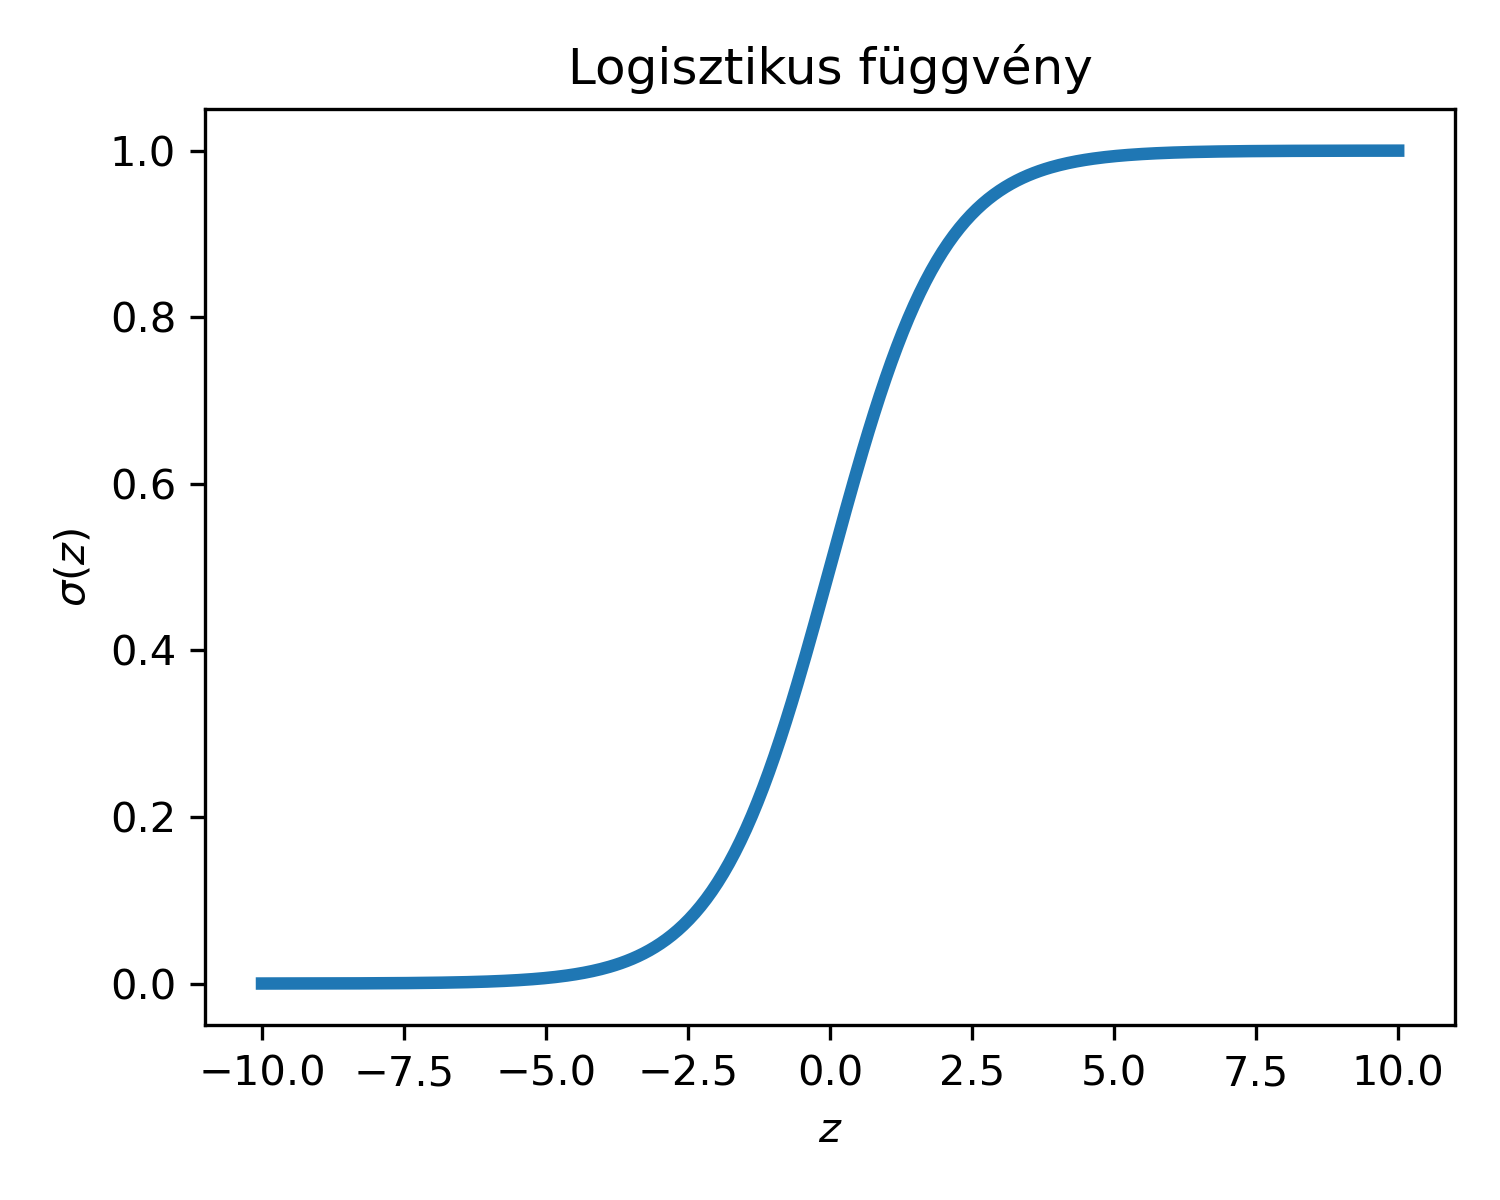
\includegraphics[width=7cm, height=7cm, keepaspectratio]{images/osztalyozas_18.png}
\end{center}
\end{column}
\end{columns}
\end{frame}

\begin{frame}{A logisztikus regresszió költségfüggvénye}
A logisztikus regresszió célja, hogy \textbf{magas valószínűséggel osztályozzon pozitív egyedeket és alacsony valószínűséggel osztályozzon negatív egyedeket}.\par\smallskip
A költségfüggvény egy mintaegyedre: 
\begin{block}{}
\[
J\left( \theta \right) = \begin{cases}
_{-log\left(1-\hat{p}\right)}^{-log\left(\hat{p}\right)} & _{ha\;\hat{y}=0}^{ha\;\hat{y}=1}\end{cases}
\]
\end{block}
Az összes mintaegyedre kiszámított költségfüggvény az egyedi költségfüggvények összege:
\begin{block}{}
\[
J\left( \theta \right) = -\frac{1}{n} \sum_{i=1}^n \left[ y_i \cdot log \left( \hat{p}_i \right) + \left(1 - y_i \right) \cdot log \left( 1 - \hat{p}_i \right) \right]
\]
\end{block}
A költségfüggvény konvex, de nem létezik a minimum megtalálására zárt formájú számítás. Ennek megfelelően a minimum közelítése iteratív algoritmusokkal lehetséges.
\end{frame}

\section{Modellezés}

\begin{frame}
\tableofcontents[currentsection]
\end{frame}

\begin{frame}{Írisz adathalmaz}
A következő példában a minta adathalmaz Írisz virágokról tartalmaz információkat. Az adathalmazban található oszlopok a virág fajtája (Setosa, Versicolor, Virginica) a csészelevelek hossza és a sziromlevelek hossza. 
\begin{center}
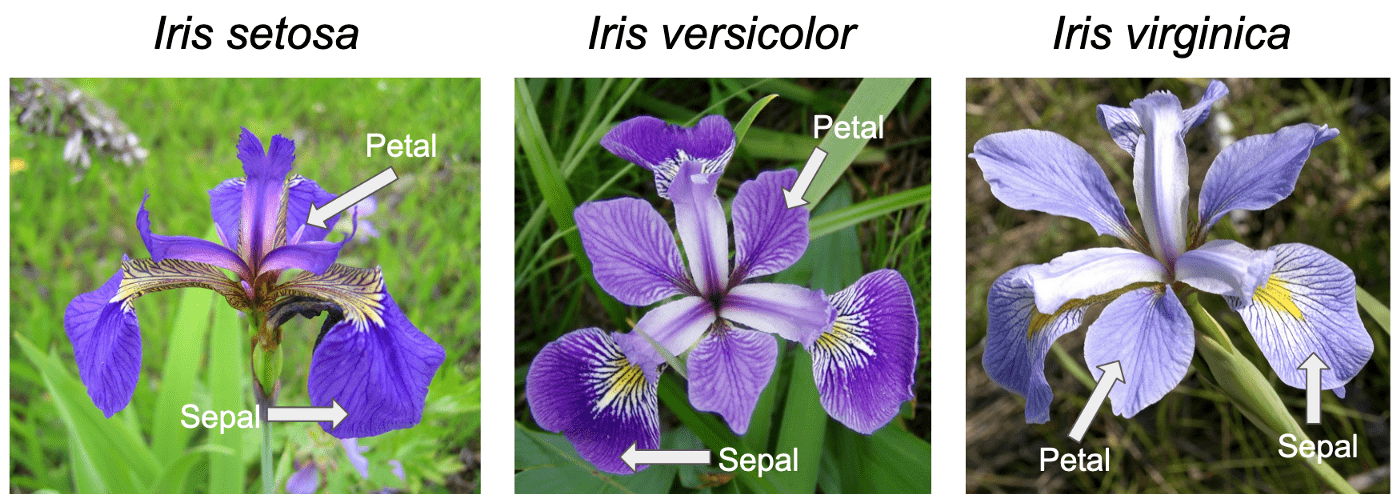
\includegraphics[width=12cm, keepaspectratio]{images/osztalyozas_19.png}
\end{center}
\end{frame}

\begin{frame}{Logisztikus regresszió az Írisz adathalmazon}
A következő példában egy bináris osztályozás a feladat. A \textbf{logisztikus regresszió eredménye egy 1D döntési határ}.\par\smallskip
Az Iris Virginica sziromszélességei 1.4-től 2.5cm-ig terjednek, míg a többi Iris virág szirmai 0.1 és 1.8cm közöttiek. A döntési határ 1.65cm körül húzódik. 2cm fölött a modell egészen biztos benne, hogy Virginicáról van szó, 1cm alatt szinte biztos benne, hogy nem tartozik az osztályba.\par\smallskip
\begin{center}
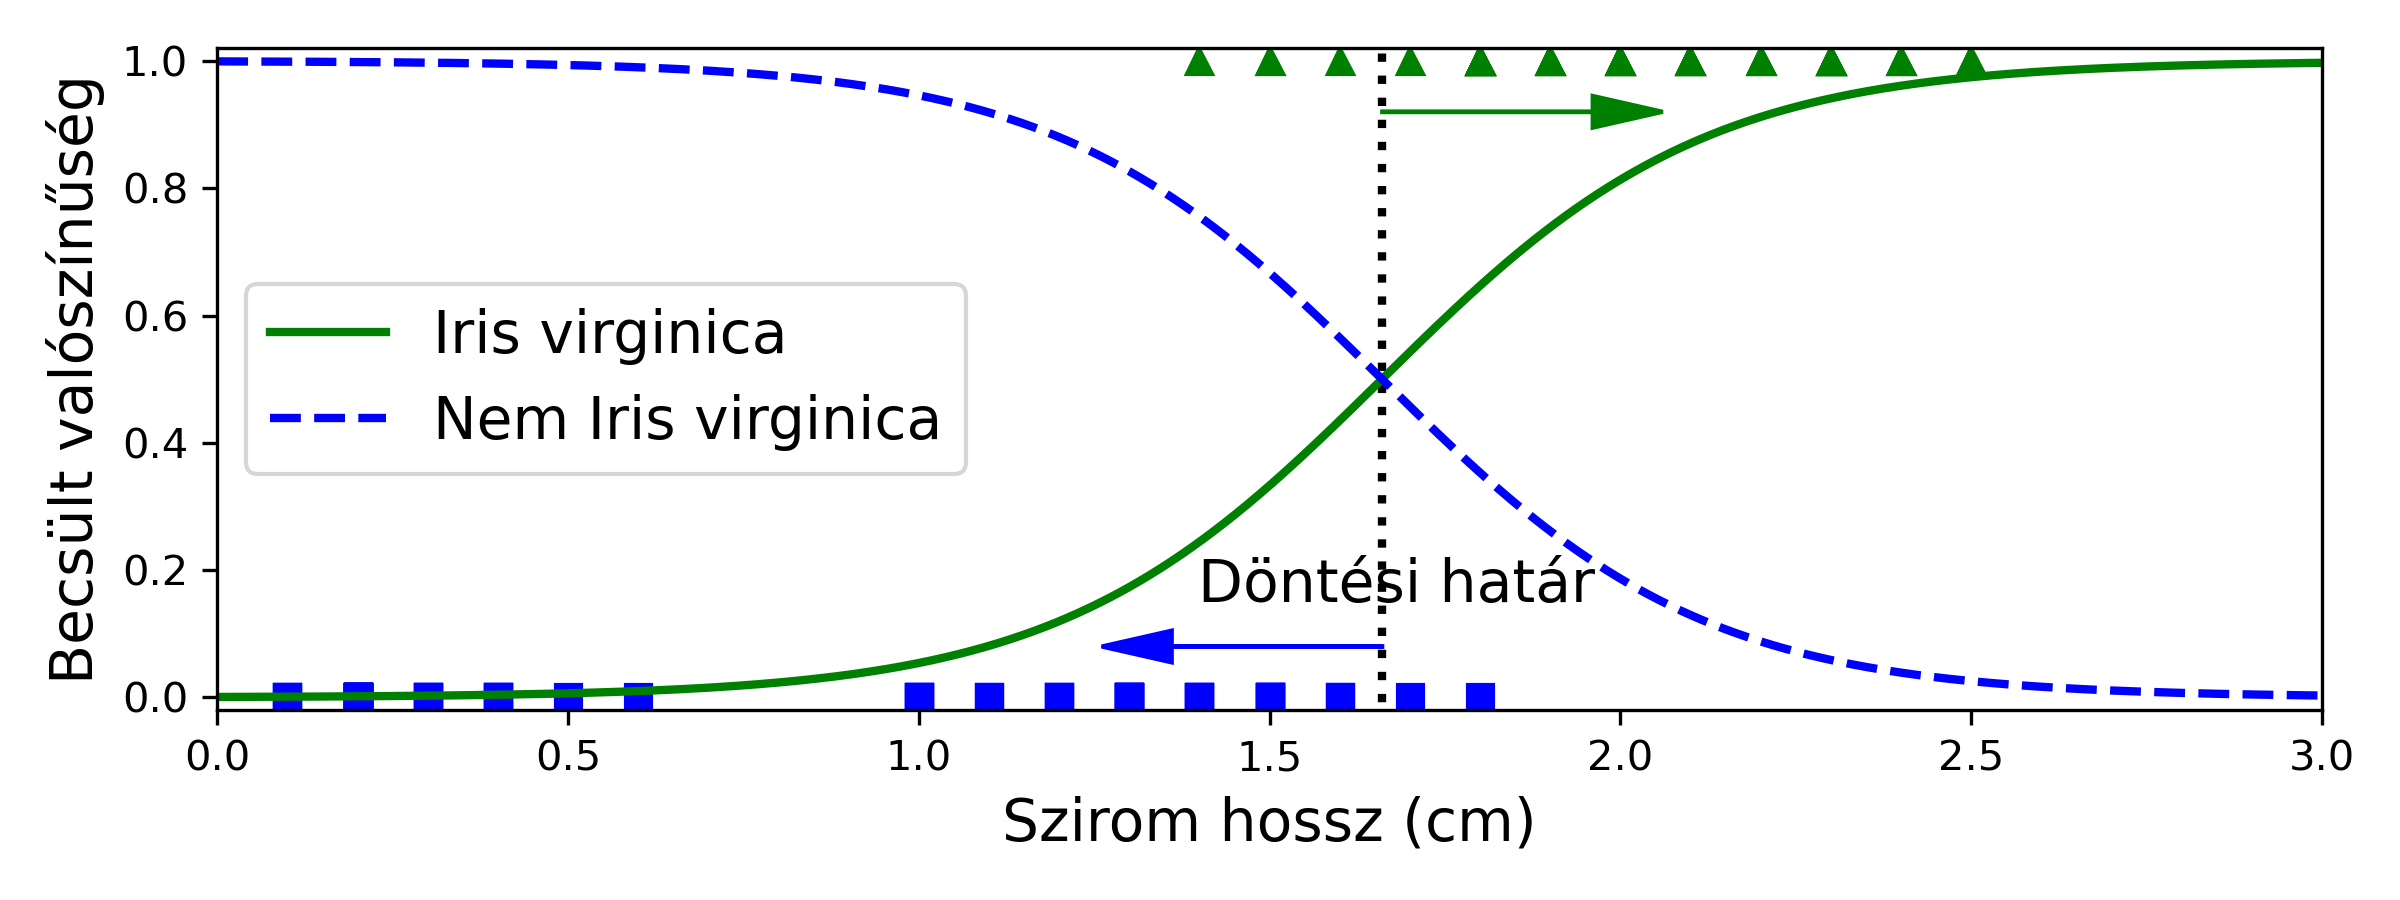
\includegraphics[width=11cm, height=7cm, keepaspectratio]{images/osztalyozas_20.png}
\end{center}
\end{frame}

\begin{frame}{Logisztikus regresszió több változóval}
Ha több $x$ változó alapján történik a modellezés, a döntési határ is több dimenziós lesz. Az alábbi példában a szirom szélesség és a szirom hossz alapján készült a becslés.\par\smallskip
Ebben az esetben a becsült valószínűség a 3. dimenzió és a határ ott húzódik, ahol a becsült valószínűség megegyezik a küszöbértékkel, tehát $\hat{p} = \theta$.
\begin{center}
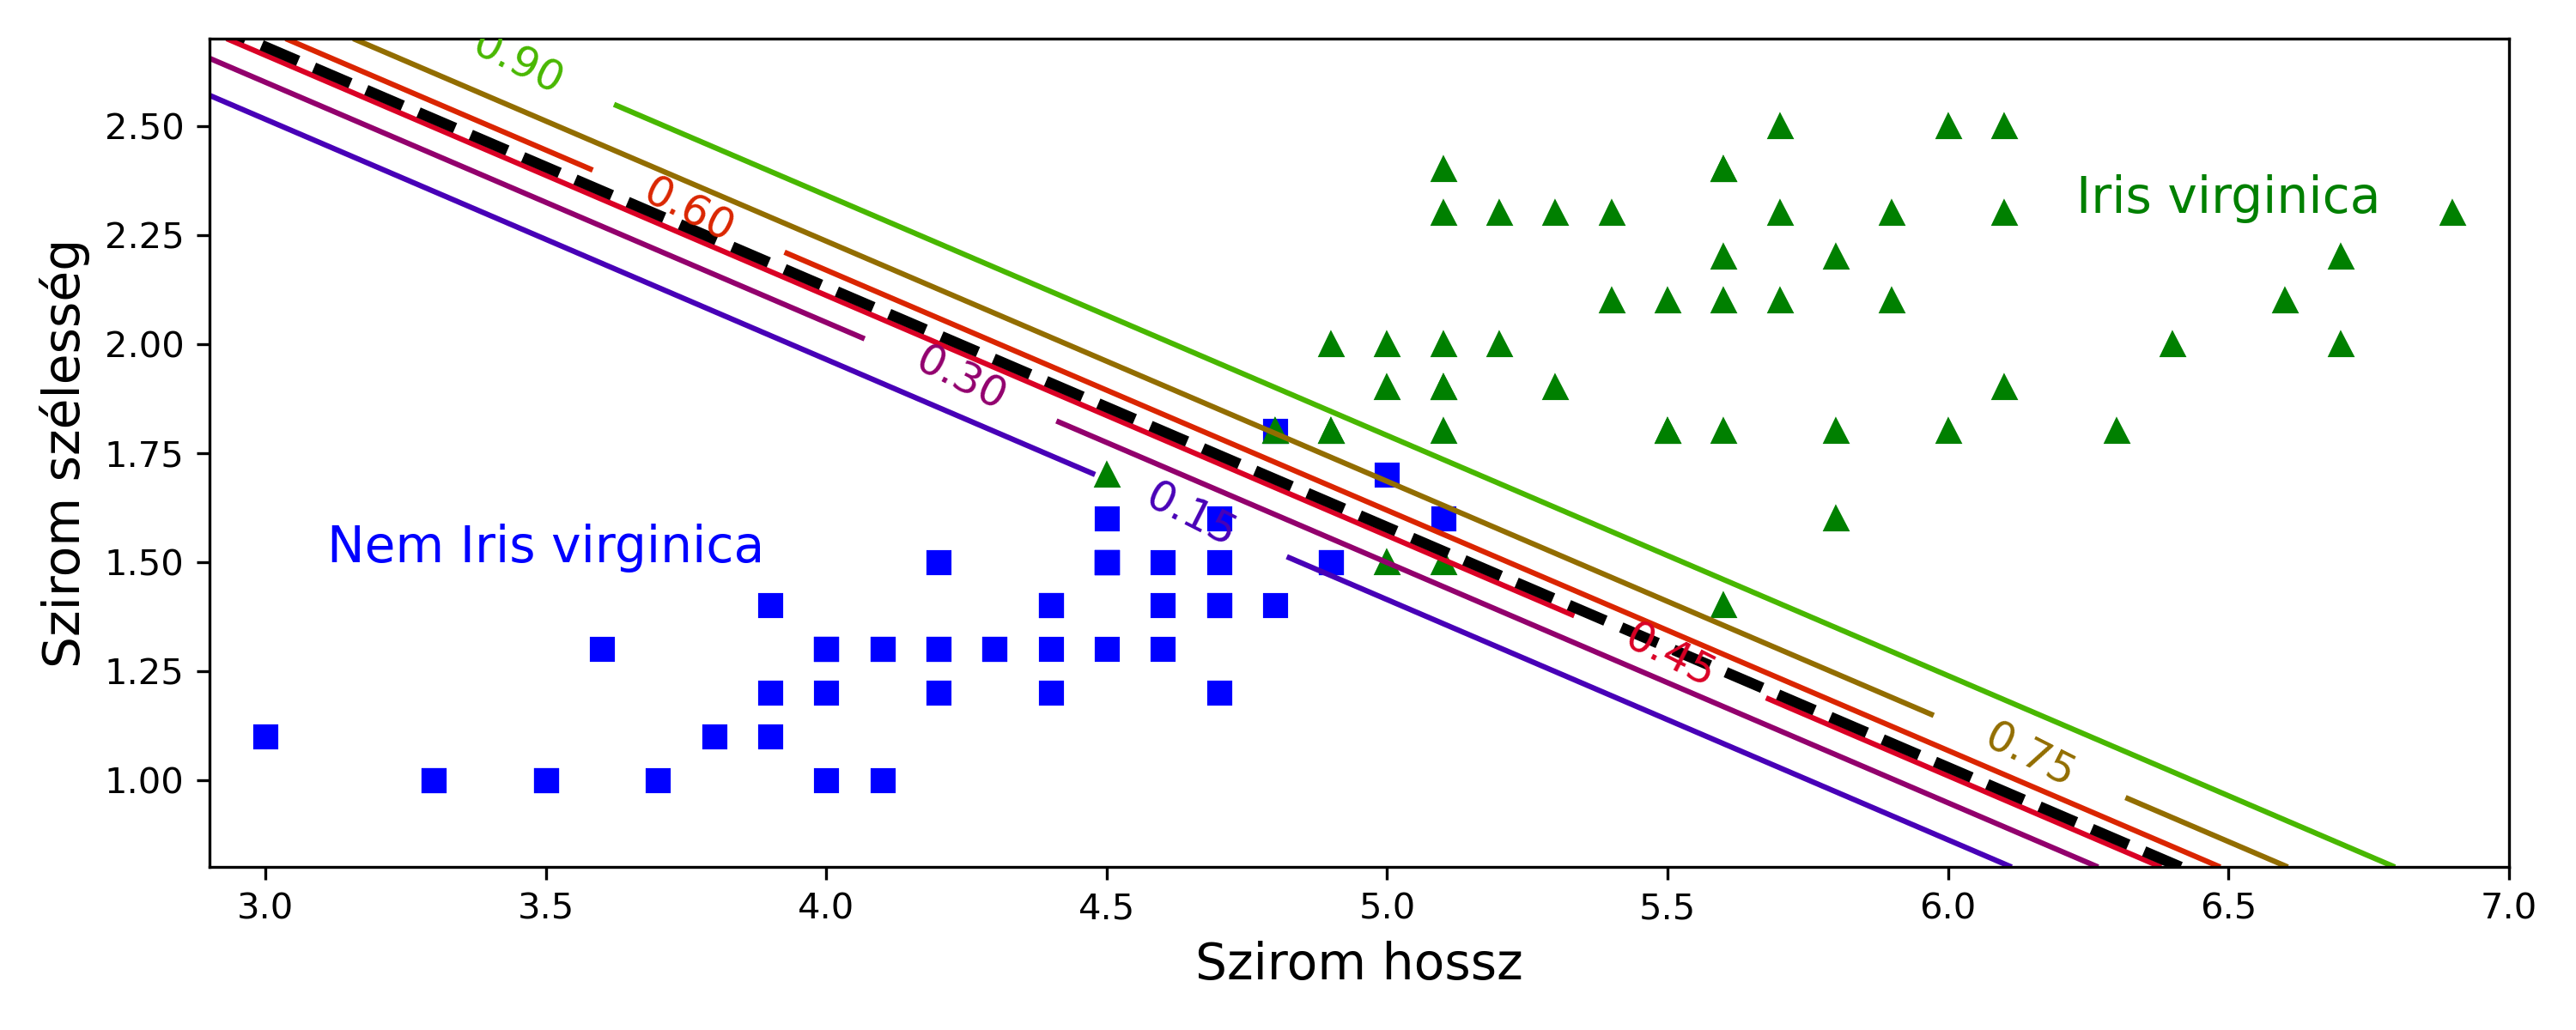
\includegraphics[width=11cm, keepaspectratio]{images/osztalyozas_21.png}
\end{center} 
\end{frame}

\section{Softmax regresszió}

\begin{frame}
\tableofcontents[currentsection]
\end{frame}

\begin{frame}{Softmax regresszió}
\begin{columns}
\begin{column}{.5\textwidth}
A logisztikus regresszió általánosítható tetszőleges számú ($k$) osztályra. \textbf{Ebben az esetben a modell azt becsüli meg, hogy mekkora valószínűséggel tartozik az egyed az adott osztályokba}.\par\smallskip
Adott $k$ osztályra számított beletartozási valószínűség: 
\begin{block}{}
\[
\hat{p}_k = \sigma \left( s \left( x \right) \right)_k = \frac{e^{x^T \theta_k}}{\sum_{j=1}^k e^{x^T \theta_j}}
\]
\end{block}
Ahol $\sigma$ a logisztikus függvény és $\theta_k$ pedig $k$ osztály tanítható paraméter vektora. 
\end{column}
\begin{column}{.5\textwidth}
Miután a modell kiszámolta, hogy $x$ mintaegyed mekkora valószínűséggel tartozik minden osztályba, \textbf{kiválasztja ezek közül a legnagyobb becsült valószínűséghez tartozót, és ez lesz a becsült érték}:
\begin{block}{}
\[
\hat{y} = \underset{k}{argmax}\left( \sigma \left( s \left( x \right) \right)_k \right)
\]
\end{block}
Az $argmax$ operátor a változónak azt az értékét téríti vissza, amelyik maximalizálja az adott kritériumot. Ebben az esetben a kritérium a legnagyobb valószínűség.
\end{column}
\end{columns}
\end{frame}

\begin{frame}{Softmax regresszió az Írisz adathalmazon}
A kép a létrejövő döntési határokat mutatja. Érdemes megfigyelni, hogy az osztályok között létrejövő döntési határok lineárisak. A görbe vonal az ábrán a Versicolor osztályhoz tartozó valószínűség.
\begin{center}
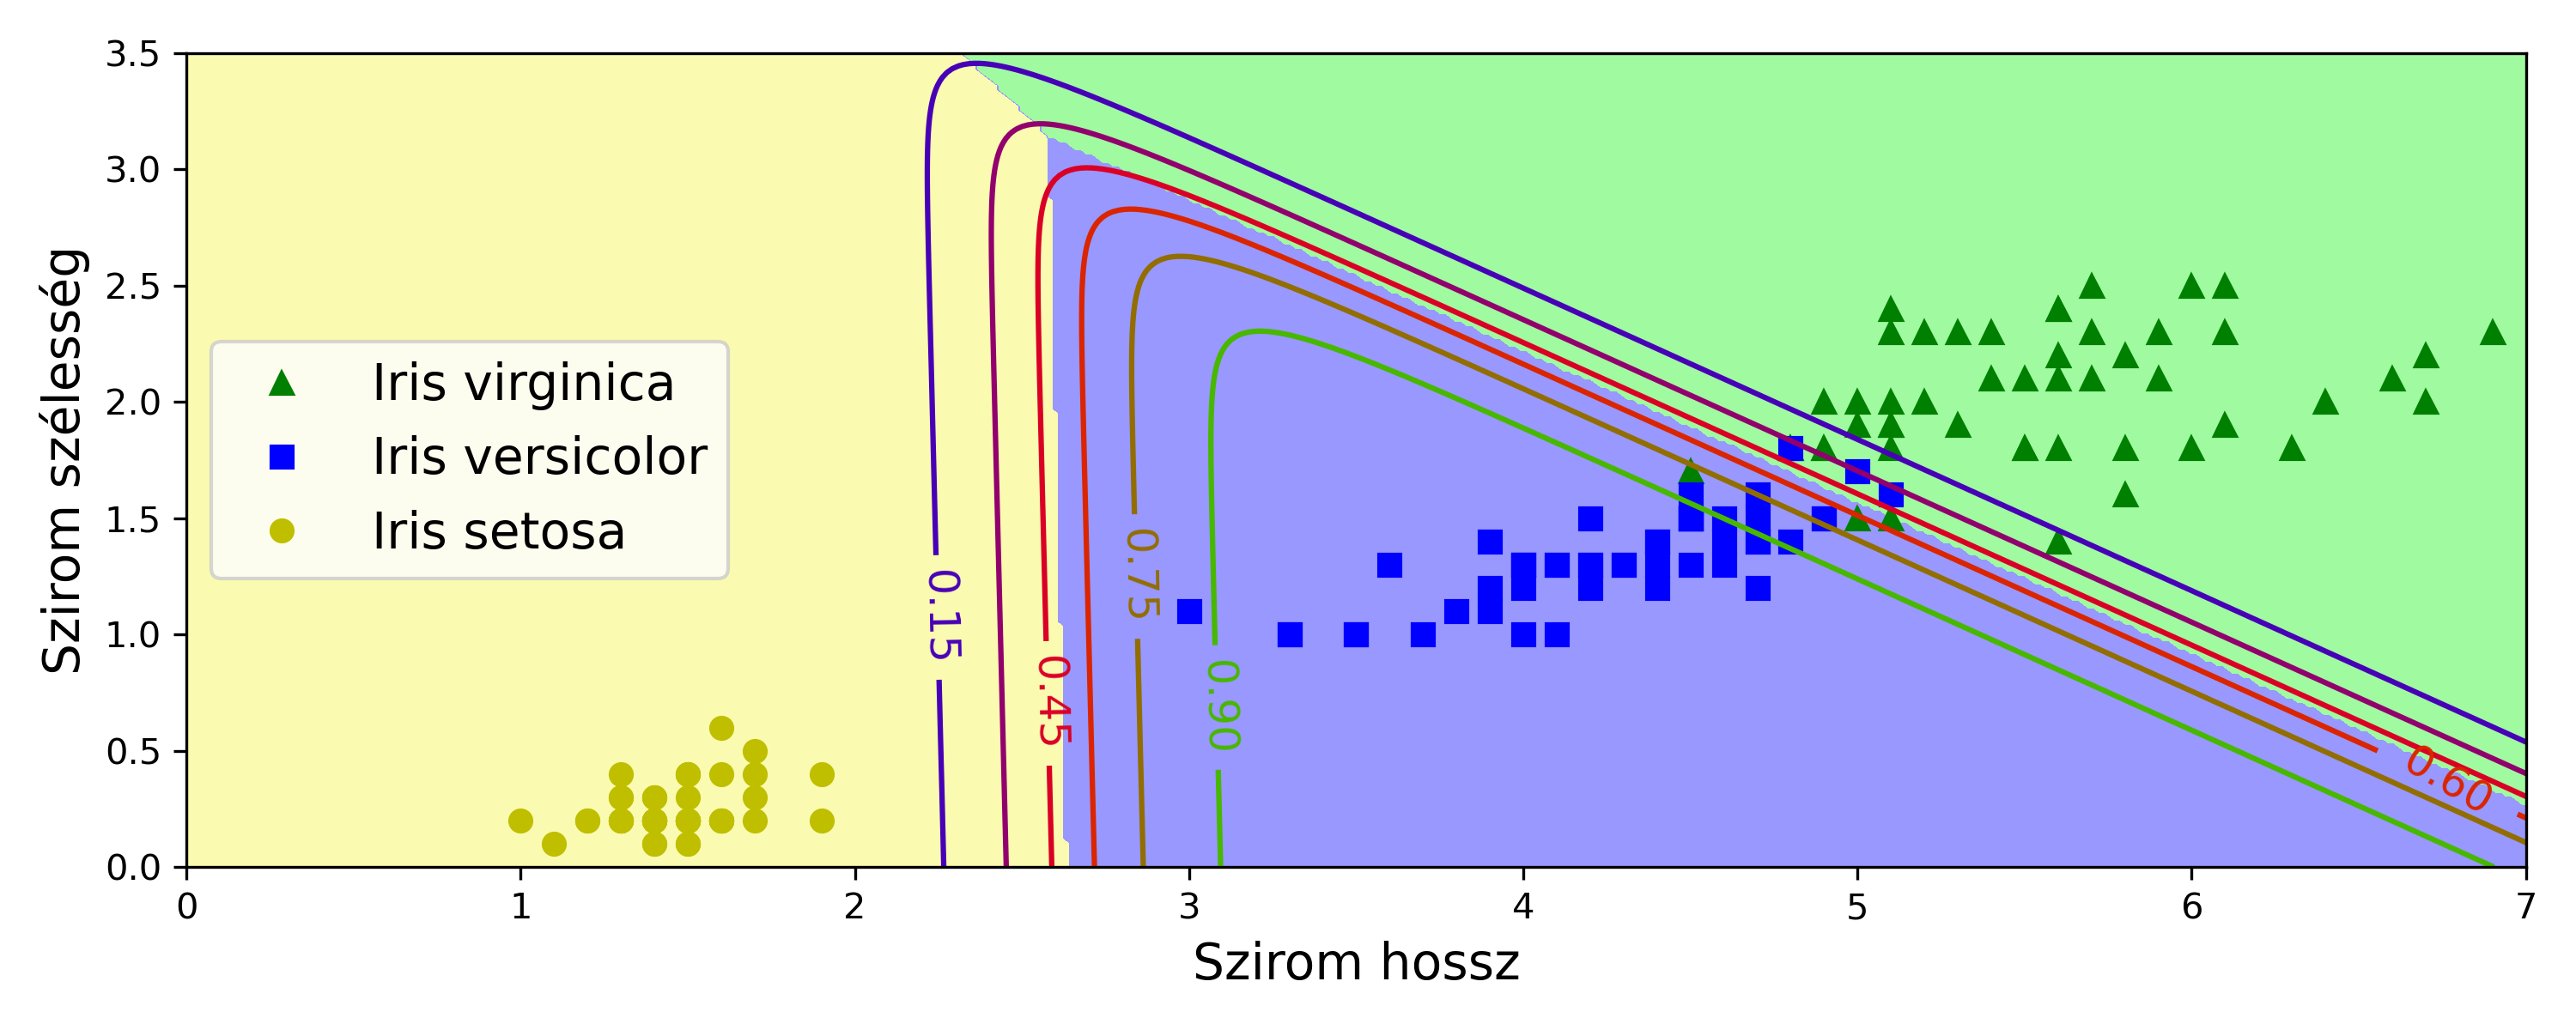
\includegraphics[width=11cm, height=7cm, keepaspectratio]{images/osztalyozas_22.png}
\end{center}
\end{frame}

\end{document}





















